%# -*- coding: utf-8-unix -*-
%%==================================================
%% thesis.tex
%%==================================================

% 双面打印
\documentclass[master, openright, twoside]{sjtuthesis}
% \documentclass[bachelor, openany, oneside, submit]{sjtuthesis}
% \documentclass[master, review]{sjtuthesis}
% \documentclass[%
%   bachelor|master|doctor,	% 必选项
%   fontset=fandol|windows|mac|ubuntu|adobe|founder, % 字体选项
%   oneside|twoside,		% 单面打印,双面打印(奇偶页交换页边距,默认)
%   openany|openright, 		% 可以在奇数或者偶数页开新章|只在奇数页开新章(默认)
%   english,			% 启用英文模版
%   review,	 		% 盲审论文,隐去作者姓名、学号、导师姓名、致谢、发表论文和参与的项目
%   submit			% 定稿提交的论文,插入签名扫描版的原创性声明、授权声明 
% ]

% 逐个导入参考文献数据库
\addbibresource{bib/thesis.bib}
% \addbibresource{bib/chap2.bib}
\begin{document}

%% 无编号内容:中英文论文封面、授权页
%# -*- coding: utf-8-unix -*-
\title{线程放置策略对层级锁性能和长期公平性影响研究}
\author{赵鹏飞}
\advisor{李健副教授}
% \coadvisor{某某教授}
\defenddate{2019年1月4日}
\school{上海交通大学}
\institute{某某系}
\studentnumber{116037910055}
\major{软件工程}

\englishtitle{Research of Influence of Threads Placement Strategy on Performance and Long-term Fairness of Hierarchical Locks}
\englishauthor{\textsc{Pengfei Zhao}}
\englishadvisor{Prof. \textsc{Jian Li}}
% \englishcoadvisor{Prof. \textsc{Uom Uom}}
\englishschool{Shanghai Jiao Tong University}
\englishinstitute{\textsc{School of Electronic Information and Electrical Engineering} \\
  \textsc{Shanghai Jiao Tong University} \\
  \textsc{Shanghai, P.R.China}}
\englishmajor{Software Engineering}
\englishdate{Dec. 17th, 2018}


\maketitle

\makeatletter
\ifsjtu@submit\relax
	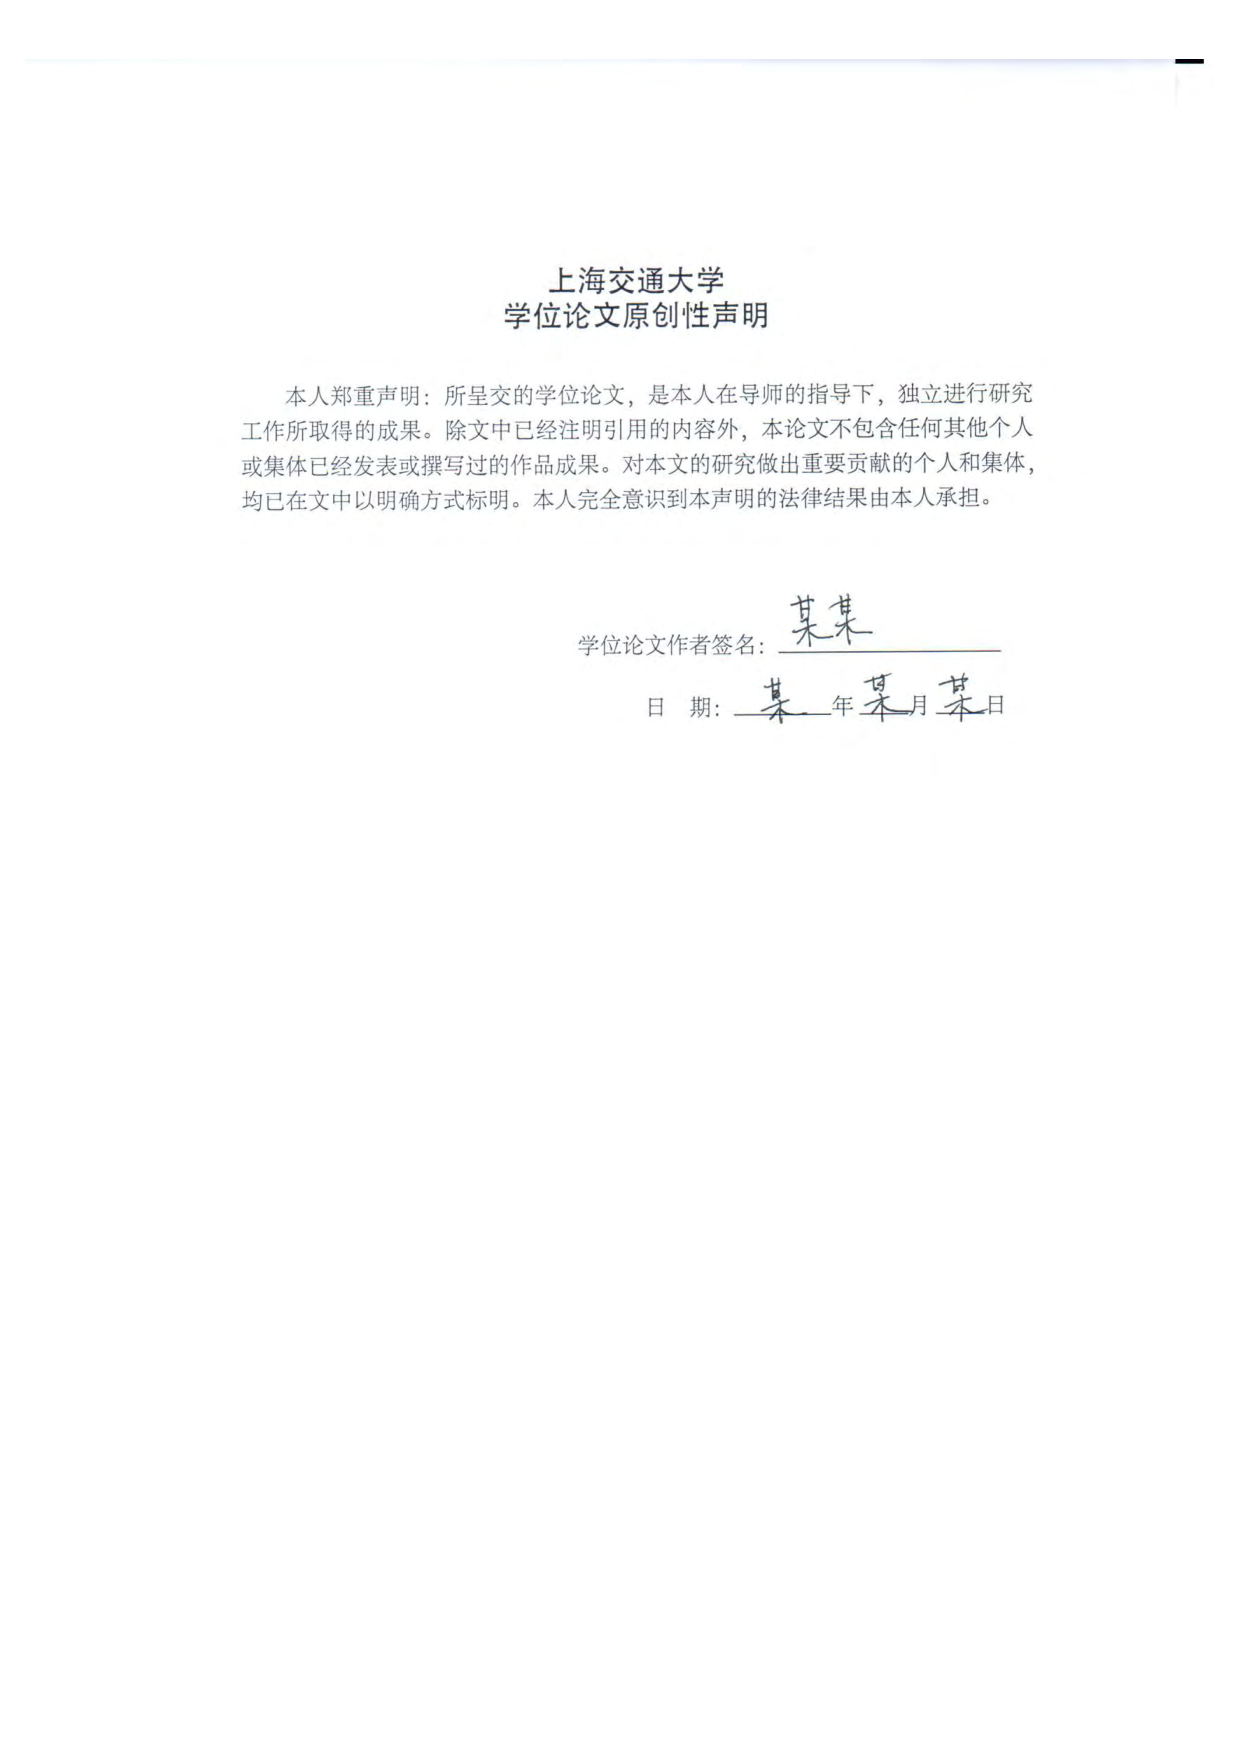
\includepdf{pdf/original.pdf}
	\cleardoublepage
	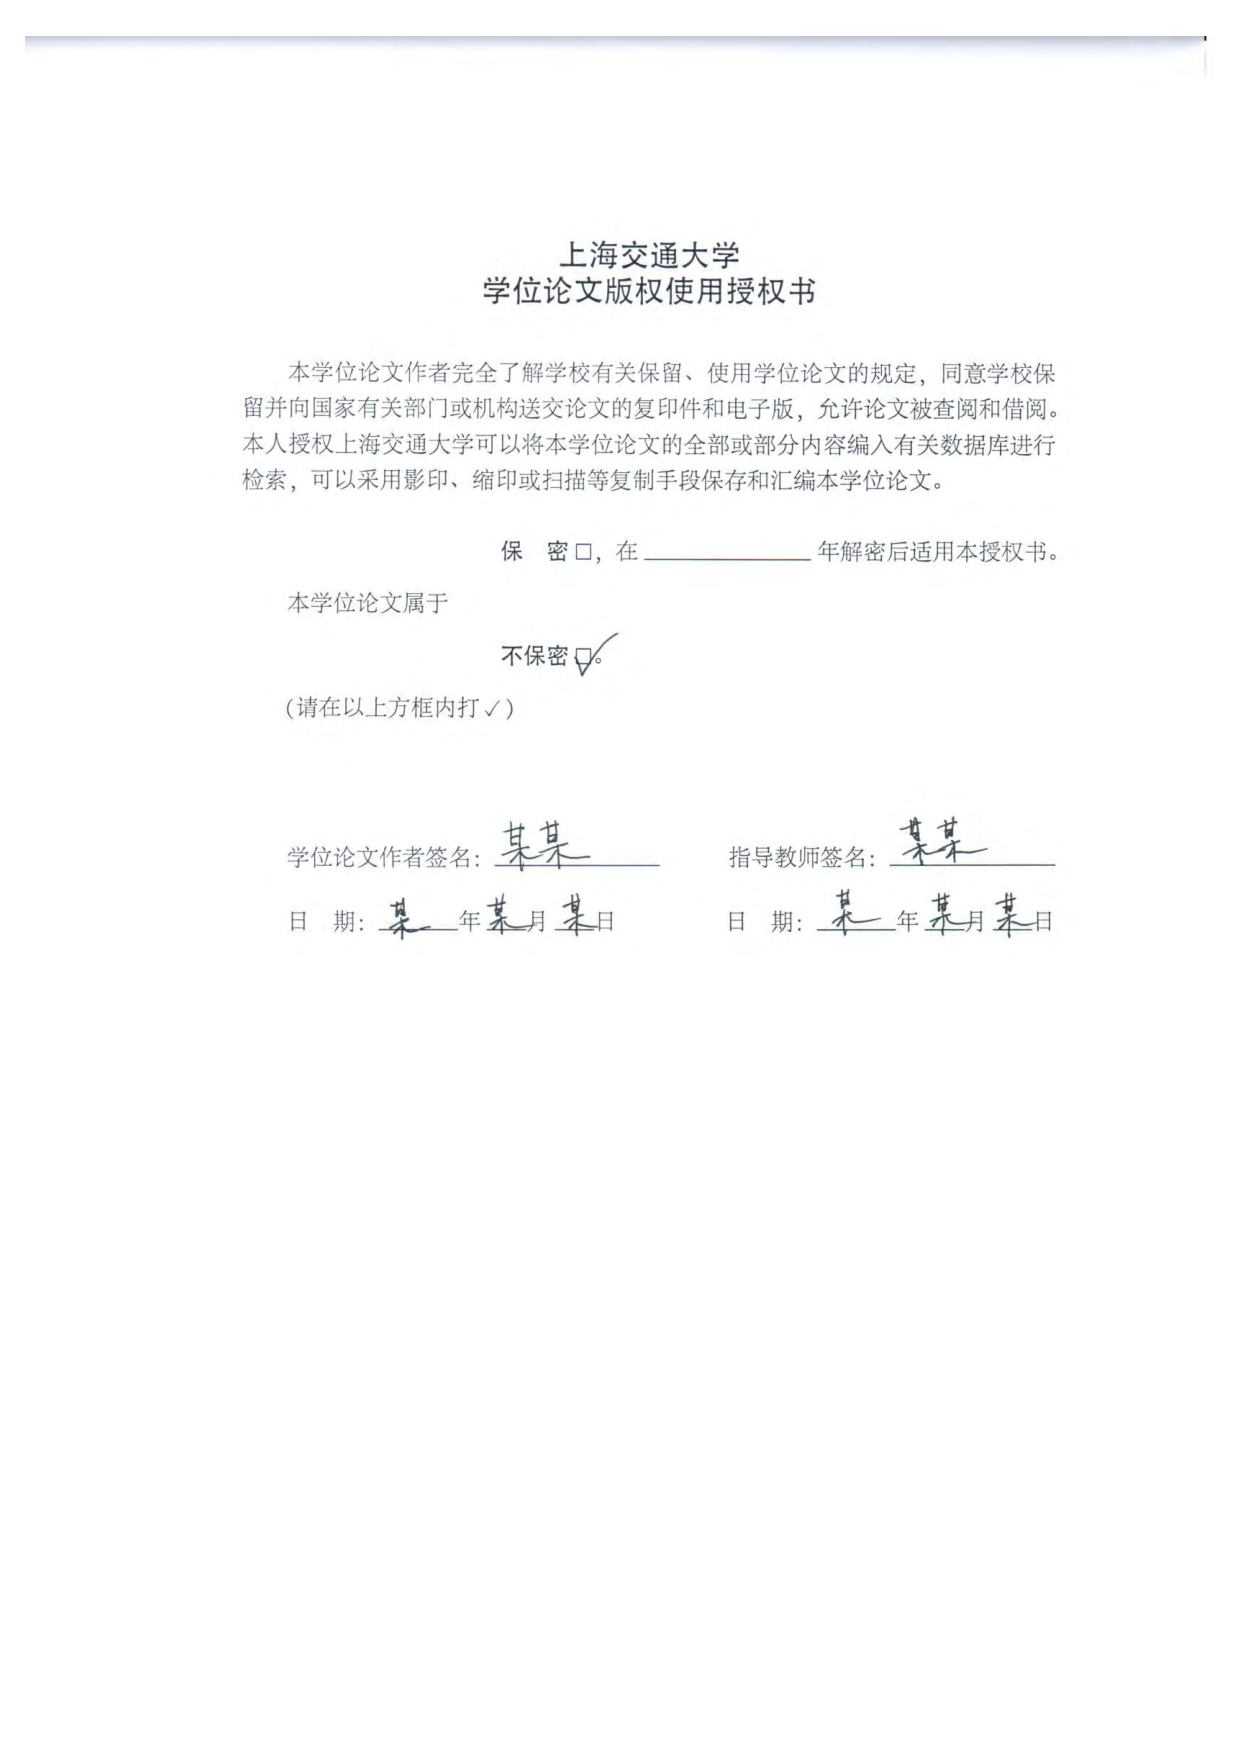
\includepdf{pdf/authorization.pdf}
	\cleardoublepage
\else
\ifsjtu@review\relax
% exclude the original claim and authorization
\else
	\makeDeclareOriginal
	\makeDeclareAuthorization
\fi
\fi
\makeatother


\frontmatter 	% 使用罗马数字对前言编号

%% 摘要
\pagestyle{main}
%# -*- coding: utf-8-unix -*-
%%==================================================
%% abstract.tex for SJTU Master Thesis
%%==================================================

\begin{abstract}
NUMA(Non-Uniform Memory Access, 非一致性内存访问)架构的出现和普及克服了SMP(Symmetric Multi-Processor,对称多处理器)架构在扩展性方面的局限性,使得单台机器上能够容纳更多的计算核心,同时NUMA架构中物理内存的分布式设计也使得访存操作具有非一致性时延的特征。一方面,更多的计算核心使得共享内存的高并发应用能够生成更多的线程并将其分布到所有的核上来充分利用多核资源提高系统吞吐率;另一方面,内存及缓存的非一致性访问特性也使得挖掘和利用共享数据的局部性成为多线程应用获取更高性能的关键。对于极易成为系统性能和扩展性瓶颈的锁来说,线程数的增多和访存的非一致性特征都对其的设计和改进提出了新的挑战。

基于队列的锁,尤其是MCS锁\footnote{命名来源于其作者名字首字母:John Mellor-
Crummey和Michael Scott}和CLH锁\footnote{命名来源于其作者名字首字母:Craig、Landin 和 Hagersten},由于其在性能、可扩展性和公平性方面的良好表现,广泛应用于很多锁集中的高性能系统。这些基于队列的锁通过将参与锁竞争的线程按照其请求锁的顺序排成一个先入先出(FIFO,First In First Out)的队列,每个线程在在队列中各自的内存位置自旋等待锁并且按照其在队列中的顺序依次进入关键区域。FIFO的队列保证了基于队列的锁的公平性,而每个线程在不同的内存位置自旋使其能提供良好的性能和可扩展性。在NUMA架构的机器上,为了充分利用多核资源,竞争同一个锁的线程不可避免地要分布在不同的NUMA节点(node)上,从而产生了跨NUMA节点的锁传递,而访存非一致性特征使得跨节点的锁传递时延通常远大于同一节点内的锁传递时延。传统的基于队列的锁由于不能感知到底层NUMA的特征并且要保持FIFO的锁传递顺序,所以产生了大量的跨节点锁传递,进而产生性能严重下降的问题。

为了解决基于队列的锁在NUMA架构下出现的性能下降问题,NUMA感知的基于队列的层级锁(以下简称层级锁),例如Cohort锁、HMCS(Hierarchical MCS)锁,改变了基于队列的层级锁全局FIFO的锁传递顺序,通过NUMA感知的锁调度使得锁尽可能地在同一个NUMA节点内的线程间按FIFO的顺序传递,只有当当前节点内没有请求者或者锁在当前节点内的传递次数超过一定限度时才将其传给其他节点内的线程,从而减少锁的跨节点传递比例,改善其在NUMA架构下的性能。由于层级锁高性能的获取要依赖于线程在NUMA节点上的分布,因此线程的放置策略对于其最终能达到的性能改善程度有很大影响。现有层级锁中线程通常会被紧凑(Compact)地放置在尽可能少的节点上来减少锁的跨节点传递,这种线程放置策略有利于层级锁挖掘和利用局部性获取更高的性能,但是层级锁优先本地传递的传递机制使得其不能保证长期公平性。除此以外,将线程平均(Even)放置在所有节点上理论上能够保证层级锁的长期公平性,但是由于线程分布较为分散所以在锁的竞争不是很激烈的时候相比紧凑放置又会存在严重的性能下降问题。

现有的简单单一的线程放置策略难以在竞争状况复杂多变的应用中同时保证层级锁的高性能和长期公平性,而对于公有云等应用场景来说,性能和公平性是缺一不可的。在这篇文章中我们提出了一种竞争感知的混合线程放置框架(Contention-Aware Hybrid Threads Placement Framework,以下简称CAH)。在CAH中我们提出了两种新的线程放置策略:有轮换的紧凑放置(Compact With Shift,以下简称CWS)和加强的平均放置(Enhanced Even,以下简称EE)。CWS在紧凑放置的基础上引入了一种轻量级的线程轮换(shift)机制来以极小的性能损失为代价抹平线程之间的吞吐率差异从而使得其能够保证层级锁的长期公平性;EE在平均放置的基础上限制其所能使用的节点数为能放下所有线程的最小节点数而不是所有节点从而在保证长期公平性的前提下尽可能地提高性能。CAH本质上是基于CWS和EE的,能根据应用中层级锁的竞争状况动态调整线程放置策略的一种混合解决方案。它通过定期地取样每个线程的锁相关的事件来评估当前层级锁的竞争状况,并且结合当前的线程数量及其分布来调节线程的放置策略,在层级锁的竞争强度足够高的时候应用EE策略,否则应用CWS策略,从而不论锁的竞争强度如何变化都能以最小的额外代价来同时保证吞吐率和长期公平性。

\keywords{\large 层级锁 \quad 竞争感知的 \quad 长期公平性}
\end{abstract}

\begin{englishabstract}
The emergence of NUMA(Non-Uniform Memory Access) architecture overcomes the scalability limits of SMP(Symmetric Multi-Processor) architecture, enabling more cores integrated on a single machine. While the distributed design of physical memory in NUMA architecture makes memory access suffer from non-uniform latency. More cores enable multithreading applications to use more threads to take advantages of multicore resources and non-uniform memory access latency makes exploiting locality more important to achieve higher performance. Both of these changes in multithreading applications pose new challenges to the design of locks, which tend to become the bottleneck of system performance.

Queue-based locks, especially MCS lock\footnote{after the initials: John Mellor-
Crummey and Michael Scott} and CLH lock\footnote{after the initials:Craig、Landin and Hagersten}, are widely used in lock-intensive high-performance systems due to their good performance on throughput, scalability and fairness. These locks push threads contending for the same lock into a first-in first-out (FIFO) queue by their requesting order. Each thread spins on its own record in the queue and enters critical section by the order in the queue. The FIFO queue guarantees the fairness of queue-based locks, and each thread spinning on a different memory location provides good performance and scalability. On NUMA architecture, in order to make full use of multi-core resources, threads competing for the same lock are inevitably distributed on different NUMA nodes, resulting in inter-node lock transfer, which typically takes much longer time than lock transfer in the same node. The traditional queue-based locks are unaware of  the underlying NUMA factor and they need to maintain the FIFO lock acquisition order. Which involves enormous inter-node lock transfers and thus causes performance degradation.


To avoid performance degradation of queue-based locks on NUMA architecture, NUMA-aware queue-based hierarchical locks (hereinafter referred to as hierarchical locks), such as Cohort locks and HMCS (Hierarchical MCS) locks, change the global FIFO lock transfer order and prefer to transfer the lock to a local waiter in the same node, only if these is no local waiter or the lock acquisitions on local node has exceeded the predefined threshold is the lock transferred to another node. Hierarchical locks reduce the frequency of inter-node lock transfer and thus achieves higher performance under NUMA architecture. Since the high-performance of hierarchical locks depends on the distribution of threads on NUMA nodes, the threads placement strategy has a great impact on the performance improvement that could ultimately be achieved. In existing hierarchical locks, threads are usually placed compactly(Compact Placement) on as few nodes as possible to reduce the frequency of inter-node lock transfer. This strategy helps hierarchical locks exploit locality to achieve higher performance, but the local-preferred lock transfer mechanism of hierarchical locks makes it hard to guarantee long-term fairness. Besides, placing threads evenly on all nodes(Even Placement) theoretically guarantees the long-term fairness of hierarchical locks, but since the thread distribution is more sparse, when the lock contention is not high enough, it could lead to serious performance degradation compared to Compact placement.

The existing threads placement strategies in hierarchical locks could not guarantee both high throughput and long-term fairness or could only guarantee both of them when highly contended. While in some scenarios such as public cloud both throughput and fairness is key to success and the lock contention could vary from time to time. In this paper, we present a contention-aware hybrid threads placement framework CAH.   In CAH we propose two new thread placement strategies: Compact With Shift (CWS) and Enhanced Even (EE). CWS introduces a lightweight thread shifting mechanism into compact placement to smooth the throughput difference among threads. EE limits the number of nodes even placement could exploit to the minimum number of nodes that could place all threads, instead of all nodes. CAH is essentially a hybrid solution of CWS and EE that dynamically adjusts the thread placement strategy based on the lock contention in the application. When the contention level of the lock is high enough, CAH applies EE strategy, otherwise CWS strategy, so that regardless of the change of lock contention, the throughput and long-term fairness could always be guaranteed.

\englishkeywords{\large hierarchical locks, threads placement, contention-aware}
\end{englishabstract}



%% 目录、插图目录、表格目录
\tableofcontents
\listoffigures
\addcontentsline{toc}{chapter}{\listfigurename} %将插图目录加入全文目录
\listoftables
\addcontentsline{toc}{chapter}{\listtablename}  %将表格目录加入全文目录
\listofalgorithms
\addcontentsline{toc}{chapter}{\listalgorithmname} %将算法目录加入全文目录

\mainmatter	% 使用阿拉伯数字对正文编号

%% 正文内容
\pagestyle{main}
%# -*- coding: utf-8-unix -*-
%%==================================================
%% chapter01.tex for SJTU Master Thesis
%%==================================================

%\bibliographystyle{sjtu2}%[此处用于每章都生产参考文献]
\chapter{绪论}
\label{chap:intro}


\section{研究背景和意义}
近年来,NUMA(Non-Uniform Memory Access,非一致性内存访问)\cite{feliu2012understanding}\cite{dashti2013traffic}架构的服务器逐渐普及,它的出现解决了对称多处理器(symmetric multiprocessor architecture,SMP)架构在可扩展性方面的局限性\cite{pusukuri2014shuffling},所以已经成为现代服务器架构设计中的一种趋势和规范\cite{kashyap2017scalable}\cite{chabbi2016contention}\cite{chabbi2017efficient}。良好的可扩展性使得单个NUMA架构的机器上可以轻易集成更多的计算核心,更大容量的物理内存和更大的内存访问带宽。NUMA架构中计算、存储等资源被组织成若干节点(node),每个节点包括若干计算核心,一块物理内存,一个或多个内存访问控制器(memory controller)和多层缓存,计算节点之间通过高速芯片间通信介质连接。在NUMA架构的机器中,某个计算核心访问其所在的计算节点的本地内存,尤其是本地共享缓存的速度通常是访问在其他计算节点上的内存或缓存的速度的数倍,也就是说NUMA架构的机器中内存访问存在非一致性时延。另外,在同一个计算节点内部,由于缓存的的分层设计,同一个计算核心访问本地计算节点的不同层次的缓存也会有显著的非一致性时延\cite{chabbi2015high}。

对于大型内存数据库(例如Microsoft SQL server)\cite{MICROSOFT-SQL}和处理引擎\cite{SAP}\cite{zaharia2010spark}(例如spark)等通过高并发来处理大规模海量数据的应用来说,随着数据规模的指数增长,必然需要进一步地扩展,通过更高程度的并发来满足需求。而NUMA架构提供的更多的核,更大的内存容量和更大的内存访问带宽使得这些应用可以生成更多的线程,并将这些线程分布到所有的NUMA计算核心上来尽可能地利用所有NUMA节点的计算和存储资源。另一方面,NUMA架构本身存在的内存访问的非一致性时延以及NUMA节点之间的有限的带宽资源对系统的线程调度和内存管理提出了新的挑战\cite{wang2012performance}\cite{boyd2008corey}。这些共享内存的应用中线程之间通常存在大量的共享数据,数据在内存及缓存中的存储位置和及访问该数据的线程的在机器上执行位置决定了数据访问的效率,因而对于系统的整体性能有很大影响。合理的内存管理和线程调度能够充分利用数据访问的局部性提高性能,而不合理的内存管理和线程调度策略可能会造成整体性能的严重损失。

通过挖掘应用的数据访问特征,比如线程线程和线程之间的数据共享范围和共享频率来建立线程之间的亲和性(thread affinity)及线程与数据之间的亲和性(data affinity)\cite{diener2014kmaf}\cite{azimi2009enhancing}\cite{tikir2008hardware},然后将共享数据多共享频率高的线程对调度到相同的NUMA节点上,同时将其最常访问的数据也放置在该NUMA节点上,可以充分利用数据访问的局部性来减少数据拷贝,减少缓存更新、增加缓存的利用率和命中率,降低数据访问延迟,进而提高应用的整体性能\cite{chishti2005optimizing}。除了将数据迁移到经常访问其的NUMA节点(co-location)外,通过分析数据本身的特征,比如读写比、共享范围、访问来源(来自于哪个NUMA节点)等,并且考虑NUMA节点间高速通信介质的数据传输压力及NUMA节点上内存控制器访问压力等因素后,还可以通过其他的内存管理方式来提高系统性能\cite{dashti2013traffic}\cite{molka2011memory},比如对于共享范围很大的只读数据或者读写比非常高的数据可以通过在NUMA节点之间复制(replication)该数据来减少跨节点的数据访问;对于访问来源非常分散的共享热点数据可以通过将数据交织(interleaving)分布到各个NUMA节点来分摊内存控制器的访问压力;对于某些应用可以将数据放置在第一次(first-touch)访问其的线程所在NUMA节点来利用局部性等。

在线程之间所有共享的数据中,有部分特殊数据不能被多个线程同时访问因而需要一种同步机制来防止其被同时访问更新,尽管近年来事务内存(transaction memory)开始流行,但是对于多数高并发的应用来说,在高度竞争的情况下锁依然是一种最基本最重要并且广泛使用的同步机制\cite{tallent2010analyzing}\cite{johnson2010decoupling}。NUMA架构的出现对于锁的性能影响主要有三个方面:1)锁本身及其保护的数据都是线程之间的共享数据,这部分数据在所有共享数据中占比通常很小,并且通常读写比很低,所以内存管理(迁移,复制,交织等)对其性能基本没有影响,而线程调度会影响对其性能仍有重要影响;2)线程之间对于锁及其保护的数据的在时间上是不共享的,而这部分数据的访问顺序是由线程的拿锁顺序决定大的,所以通过线程调度优化锁的性能还必须考虑锁本身的传递机制;3)(互斥)锁保护的数据只能在线程间串行访问,这使得锁很容易成为应用的性能瓶颈甚至导致应用崩溃\cite{boyd2012non},NUMA因素的出现进一步加剧了这种瓶颈,也对锁的设计提出了新的挑战。

在传统的SMP架构中,基于队列的锁,例如CLH锁\cite{craig1993building}\cite{magnusson1994queue}\cite{scott2013shared}和MCS锁\cite{mellor1991algorithms}\cite{scott2013shared},广泛应用在许多锁集中的高性能系统中\cite{dice2011flat}。这些基于队列的锁将所有等待访问关键区域的线程排成先进先出(FIFO,first in first out)的队列,每个线程通过在队列中各自对应的内存位置上自旋来等待进入关键区域。相比所有线程在同一个内存位置上自旋的spin lock, FIFO的队列保证了基于队列的锁的公平性;每个线程在各自的内存位置上自旋,分散了线程对锁变量的竞争,减少了锁传递时的缓存更新,从而提能提供更好的性能和可扩展性。然而在NUMA架构中,这些基于队列的锁的性能显著下降,这主要是由NUMA架构机器的物理架构决定的,由于传统的基于队列的锁不能感知NUMA架构硬件层面的访存的非一致特性,同时为了保持先来先服务的锁传递顺序,就会产生锁在NUMA节点之间的随意传递,而锁在NUMA节点之间的传递地时延通常是在同一个NUMA节点内传递时延的数倍,从而加长锁传递的时间和关键区域的执行时间,增加时延,减小吞吐率,使得性能显著下降。

传统锁在NUMA架构上性能衰退的主要原因是跨节点的锁传递代价远高于同一节点内的锁传递代价而传统锁不能感知到底层的NUMA因素。NUMA感知的层级锁在考虑NUMA因素的情况下通过本地偏好的锁传递规则减少了锁的跨节点传递,从而改善了锁在NUMA架构下的性能表现。本文在此基础上从线程调度/放置策略的角度对现有的基于队列的层级锁的性能和其他特性(长期公平性)进行优化,使其能够更好地适应诸如公有云等对于锁的性能,公平性,可扩展性等都有很高要求的应用场景。

NUMA架构是可预见的未来大型计算机硬件架构设计的大趋势,而随着医疗,交通,社交等领域产生的大数据的爆发式的增长,以及云计算等共享计算资源模式的快速发展,大型应用对于性能,可扩展性和公平性等方面的要求必然进一步提高。本文的研究使得基于队列的层级锁能够更好地适应未来软硬件的特性和需求变化,更好地服务于当下和未来相关领域的发展。总而言之,NUMA架构的出现解决了大型计算机硬件层面的扩展性问题,使得高性能共享内存应用能够进一步地扩展来满足日益增长的数据处理的需要;层级锁的出现改善了基于队列的锁在NUMA架构下存在的性能衰退问题,但是也带来了长期公平性不足的新问题;而本文的研究从线程调度/放置的角度进一步地优化现有的层级锁设计,使其在保持性能和可扩展性的前提下在一定程度上保证公平性。考虑到NUMA架构的机器的不断普及以及发展趋势和公有云等对公平性,性能和可扩展性都有很高要求的应用场景的不断增多,本文的研究将使得层级锁能够更好适应这些应用场景的需求,并且在可预见的未来有更大应用前景。
\section{国内外研究现状}
性能和公平性是任何锁的设计中都必须要考虑的两个重要标准\cite{chabbi2015high}。一般情况下,线程执行关键区域的时间非常短,甚至可能比其拿锁的时间还要短\cite{johnson2010decoupling},所以锁传递的时延对于锁的性能尤其是在锁的竞争已经饱和的情况下的性能的影响非常大。而在NUMA架构下,访存的非一致性时延特征导致跨节点的锁传递和同一节点内的锁传递在时延方面存在数倍的差异,从而使得跨节点的锁传递比例成了影响锁性能的关键因素。针对NUMA架构下跨节点的锁传递带来的锁性能下降问题,现有的优化方案大多数本质上都是通过减少锁的跨节点传递来改善其性能的,具体分为以下四类,即委托执行,线程聚类,线程迁移,NUMA感知的层级锁。另外,应用程序在NUMA架构下的进一步扩展使得其对锁的竞争变得更加难以预测,过度的竞争反而会带来系统整体性能的下降,所以通过竞争控制也能改善NUMA架构下锁的性能。

\subsection{委托执行}
为了避免锁在NUMA节点之间传递的巨大开销,要执行关键区域的线程可以委托一个或几个专门的核代为执行\cite{oyama1999executing}\cite{lozi2012remote}\cite{fatourou2012revisiting}\cite{hendler2010flat}\cite{guiroux2016multicore},从而完全避免锁的传递所造成的缓存数据的同步及由此带来的时延增加和吞吐率损失,因为锁及其保护的数据始终在对应核的缓存中。这种方案的代价是需要额外的线程间通信并且至少需要一个专用的核专门执行关键区域。RCL(remote core locking)\cite{lozi2012remote}就是委托执行的一种,RCL的作者观察到大多数多线程应用并不需要或者不能扩展到现代多核机器的所有核上,所以让某几个特定的核专门执行关键区域既利用了空余的核又能带来潜在的性能提升,要执行关键区域的线程不需要通过竞争锁来进入关键区域,而是通过优化后的远程过程调用委托特定核完成关键区域的执行从而完全避免锁及其保护的数据的传递。委托执行本质上是在迁移关键区域的执行,相比其他锁,它能在某些特定应用中防止高度竞争情况下应用性能的崩溃,但是它最大的缺陷是需要修改使用传统锁的历史遗留代码,原有代码中的关键区域需要额外的技术和时间被识别和修改之后才能利用委托执行的的高性能。

\subsection{线程聚类}
线程聚类是把同一个应用的线程或者竞争同一个锁的线程放置到同一个NUMA节点上\cite{tam2007thread}\cite{thekkath1994impact}\cite{xian2008contention}。这样做的好处是所有的共享数据都存在于本地内存或者缓存中,并且将锁的传递限制在同一个NUMA节点内部,避免了锁在NUMA节点之间传递的开销。该方案本质上是通过建立线程间的亲和性来挖掘和利用数据访问的局部性,所以也常被用在一般的共享数据中将有共享内存数据的线程放置在同一个计算节点上来最大化缓存的共享和复用。线程聚类能显著改善线程较少的小规模应用
的性能,但是对于具有大量线程的高并发应用程序而言,其所拥有的线程数通常远大于单个节点上的计算核心,按照线程聚类的方法所有线程都会被分到一个聚类中,因而会产生负载不均衡的问题,同时并行性也被牺牲了,除此以外也会带来拿锁者被抢占或者等待者被抢占等新问题,最终的结果可能得不偿失,所以线程聚类一般只适用于线程数量较少的小规模应用。

\subsection{线程迁移}
在系统运行的同时,将锁的等待者动态地调度到锁的持有者当前所在NUMA节点上,从而减少锁及关键区域的数据在NUMA节点之间的传递\cite{sridharan2006thread}\cite{thekkath1994impact}。这种方案主要基于以下观察,即锁集中的多线程应用的性能对于线程在NUMA节点之间的分布高度敏感但是操作系统的调度器感知不到锁在线程之间的竞争自然不能将锁的竞争因素加入到调度器的调度策略中,所以线程迁移可以看作是在考虑锁竞争因素的情况下对操作系统默认调度器调度策略的一种补充。shuffling\cite{pusukuri2014shuffling}是通过线程迁移来提高锁的性能的一种,它定期地将线程按照其“到达时间”(线程请求锁的时间)来排序;然后将“到达时间”接近的线程分到同一组中,每组的线程数量大致等于单个NUMA节点上的计算核心数;最后将分到同一组的线程迁移到同一个NUMA节点上去执行。因为连续请求锁的线程被分为同一组并且放到同一个节点上执行,所以锁在节点之间的迁移频率被显著降低;另外放置在每个计算节点上的线程数不超过该节点上的计算核心数又能避免负载不均衡及抢占等问题。线程迁移能够有效减少锁及关键区域的迁移,提高系统的整体性能,并且不改变原有锁的传递顺序,代价则是较为频繁大量的线程迁移及其带来的潜在缓存污染等问题。

\subsection{NUMA感知的层级锁}
层级锁利用多层的锁来对应下层的NUMA结构,将锁的竞争分割在不同的NUMA节点或者同一个NUMA节点内部不同的计算核心上,从而减少锁及关键区域数据在NUMA节点间的随意迁移频率\cite{dice2012lock}。与其他解决方案的主要不同之处在于层级锁是对锁的调度,所以会改变原有锁的传递顺序。层级锁本质上是通过牺牲短期公平性来换取减少锁的跨节点传递频率提高锁的吞吐率的。具体来说,在层级锁中,锁的持有者会优先将锁传递给当前节点上的最早的请求者而不是所有节点范围内的最早的请求者,只有当前节点上没有请求者时才会传给其他节点上的请求者。另外为了避免饥饿(starvation)及深度不公平等问题,层级锁中通常会设定一个上限(threshold)来限制其在同一个节点内的连续传递次数。

现有的层级锁设计方案包括lock cohorting\cite{dice2012lock}, HMCS锁\cite{chabbi2015high},AHMCS锁\cite{chabbi2016contention}和HMCS-T\cite{chabbi2017efficient}等。lock cohorting的设计包括一个全局锁(global lock)和每个NUMA节点上的本地锁(local lock)。全局锁和本地锁都可以是任何传统的锁(MCS, CLH,门票锁,自旋锁等)。全局锁在所有节点之间共享,它的主要功能是将竞争分隔到各个节点之内。一个本地锁只在本地节点里边的线程之间共享并且用来同步本地节点内的线程。一个线程只有同时拿到全局锁和其所在节点的本地锁才可以访问关键区域,通常的拿锁顺序是先拿本地锁再拿全局锁。层级锁一般用在竞争线程多竞争激烈的场景中,所以大多数情况下同一个NUMA节点内的线程只需要有一个线程显式拿全局锁另一个线程显式放全局锁,其他线程直接继承全局锁。由于只有全局锁会在节点之间传递并且该传递频率因为竞争分割的关系会很低,所以锁的整体性能显著提高。

HMCS将lock cohorting的思想推广到了具有深层NUMA架构的机器中,从而使用三层甚至四层地MCS锁来潜在地发掘和利用各个NUMA层次的局部性获取更高的性能。HMCS适合竞争线程多竞争锁请求频繁的场景,但是竞争强度较小或者没有竞争的场景下,其多层的锁架构会带来较大的时延。AHMCS针对该问题使用多个互相正交的策略(事务性内存,竞争感知、动态适应的锁树等)来同时达到高竞争时的高吞吐和低竞争时的低时延。HMCS-T保持了HMCS的高性能,并且通过超时机制来使HMCS具备放弃竞争特性从而控制竞争者数量避免无意义的空转等待。由于基于队列的MCS锁相比自旋锁、门票锁等在高度竞争地场景下具有性能好,可扩展性好,并且保证公平性等优点,所有大多数层级锁中将MCS锁作为其各层的基本锁。上述层级锁具有不同的其他方面地特征和创新,但它们都是通过竞争分割降低锁的跨节点传递频率来提高锁的吞吐率的。

\subsection{竞争控制}
许多并行程序的线程之间的通信变化是不可预测的,这使得线程对于共享数据的竞争无法预测和控制,从而使得大多数情况下表现良好的锁可能因为线程对共享数据的竞争的突然加剧而性能急剧下降甚至崩溃\cite{johnson2010decoupling}\cite{boyd2012non}。在NUMA架构下,如前所述,硬件的扩展使得软件应用规模进一步加大,从而使得共享数据的竞争更加不可预测和控制,也进一步加大了应用性能下降和崩溃的风险,所以通过控制线程对于共享数据的竞争也可以改善NUMA架构下锁的性能。

F.Ryan Johnson\cite{johnson2010decoupling}认为通过自旋(spinning)能够最大化锁的性能但是会白白浪费计算资源,而基于阻塞(blocking)的方式节省了计算资源但是可能会加长关键区域的执行时间,同时在高度竞争或者负载变化的情况下,操作系统的调度造成的线程被抢占进一步加剧了上述两种竞争控制策略的缺陷。作者观察到竞争控制与线程调度或者负载管理带来的问题之间是正交的,所以将两者解耦能够更有效的解决两者带来的问题,基于此提出了一种与竞争大小相解耦的的负载控制机制来控制活跃线程数,从而能结合利用spinning的高效性和blocking大的健壮性。类似的,CST锁\cite{kashyap2017scalable}中作者认为简单的spin,block或者spin-then-block竞争控制机制都不能解决NUMA架构下锁存在的扩展性问题,因为不管哪种机制都会受到操作系统调度器的调度决策的影响,所以提出在锁传递的时候在尽可能地保证先来先服务(first-in first-out)的顺序下应该尽可能地将锁传给处于spinning状态的竞争者,从而尽可能地避免因为线程调度而加长关键区域的执行时间。

AHMCS\cite{chabbi2016contention}锁中,作者认为NUMA架构下可扩展性和性能都很好地HMCS\cite{chabbi2015high}锁不能适应竞争和负载多变的环境。HMCS锁在高竞争的情况下能够利用局部性感知提供高吞吐率,但是在竞争很小地情况下局部性感知本身没有必要而且为了进行局部性感知会造成不必要的额外时延,在此基础上作者认为局部性感知的锁应该是竞争感知的,并且提出了可以动态适应竞争变化,动态改变锁的层数的AHMCS锁,从而使其能够在高度竞争的情况下保持高吞吐率的同时在竞争强度不高时也能保证低时延。

Multhusian锁\cite{dice2017malthusian}的作者认为现代大型应用程序大多数使用了过多的线程(overthreaded),大部分这类程序中由于锁的高度竞争,过多的线程非但没有提高应用的性能,反而可能因为扩展性崩溃(scalability collapse)而造成性能衰退。作者通过实验说明了大多数应用中,随着线程数的增多,在锁饱和前性能就开始衰退了,所以使锁饱和的线程数可以用来作为竞争控制的目标。为了将线程数控制在饱和点附近,作者对MCS锁的传递机制进行了修改,借用了内存管理中的thrashing机制\cite{denning1980working}将所有线程分为了活跃态(可以请求锁)和抑制态(不能请求锁)两个集合,其中处于活跃态的线程数大约等于锁的饱和点大小,从而有效控制了竞争线程数进而保证性能不会下降太多。该方案事实上通过牺牲MCS锁的短期公平性来放置性能下降,为了保证长期公平性,作者使用了shift机制来在两个集合之中循环移动线程。

\section{研究内容和结构安排}
本文的研究在基于队列的层级锁基础上,针对现有层级锁中的简单单一的线程放置策略不能在锁的竞争复杂多变的情况下同时保证其性能和长期公平性的缺陷,提出了一种新的竞争感知的混合线程放置框架,使得基于队列的层级锁能够在竞争状况变化的情况下以尽可能小的代价同时达到高性能和保证长期公平性。


\subsection{竞争感知的混合调度框架}
性能和公平性是任何锁设计中最重要的两个指标,而目前的层级锁设计及其线程放置策略或者不能保证最佳的性能,或者不能保证线程之间的长期公平性,或者只能在高竞争的情况下同时保证性能和公平性。究其原因主要有两点:1)现有部分线程放置策略没有考虑对性能和长期公平性都有很高要求的应用场景;2)简单单一的线程放置策略难以满足复杂多变的应用竞争状况。对于公有云等很多应用场景来说,为了给用户提供按需付费的服务并且高效地利用计算、存储等资源,性能和公平性对于其的成功都是至关重要的\cite{rao2014towards};另外,很多大型应用中线程之间对于共享资源的竞争是不可预测和控制的,通常情况下竞争很小的一块共享数据可能会突然变得高度竞争,比如搜索引擎中突然出现的热门事件的搜索\cite{chabbi2016contention}。所以为了适应这些复杂应用场景的需求,现有的基于队列的层级锁的线程放置策略必须要先解决上述两个缺陷/挑战。

基于此,本文的研究首先针对紧凑放置不能保证长期公平性和平均放置性能较差的问题对其分别做了改进,对应得到以下两种新策略,加强的平均放置(Enhanced Even,EE)和有轮换的紧凑放置(Compact With Shift,CWS)
\begin{itemize}
\item 加强的平均放置。为了尽可能地保证平均放置的性能,我们限制该策略所能使用的NUMA节点数为能满足需要的最少的节点数,而不是全部可用的节点数。相比原有的平均放置策略,新的策略在保证长期公平性的同时尽可能地保存局部性使得层级锁能尽可能地挖掘局部性从而保证高性能,然而相比紧凑放置,新的策略在某些情况(竞争强度不足)下还是会有相当的性能损失。
\item 有轮换的紧凑放置。我们发现紧凑放置之后每个线程的吞吐率是由其所运行的位置决定的,所以在紧凑放置的基础上,引入了轮换(shift)机制,即通过定期地交换线程的位置来抹平线程的吞吐率之间的差异从而保证长期公平性。在有轮换的紧凑放置策略中,轮换的频率决定了最终的长期公平性的好坏。
\end{itemize}
基于上述两种改进后的策略及应用程序竞争状况复杂多变的特征,我们提出了竞争感知地混合线程放置框架(Contention-Aware Hybrid Thread Placement Framework)CAH。相比现有的简单单一的线程放置策略,CAH主要有以下几个特征:
\begin{itemize}
\item 竞争感知,该框架通过取样检测锁事件来评估当前的竞争状况,从而能够适应复杂多变的程序竞争状况。其中锁事件是每个线程与锁相关的操作(请求锁,拿锁,放锁)。
\item 混合,该框架可以被看作是有轮换的紧凑放置和加强的平均放置的混合体,在竞争强度足够的情况下应用加强的平均放置否则应用有轮换的紧凑放置策略,最终的目的是用最小的代价同时保证层级锁的性能和长期公平性。
\item 动态,该框架按照应用中层级锁的复杂多变的竞争状况动态地应用合适的线程放置策略。
\end{itemize}

在特定应用中特定的竞争状况下,为了确定一个最合适线程放置策略,我们从Malthusian锁中引入了饱和点(saturation point)的概念。饱和点是能保证某个线程放锁时总有至少一个其余线程在等锁的最小线程数。我们的线程放置框架偏向于应用加强的平均放置策略,因为相比有轮换的紧凑放置策略它没有额外的线程迁移开销。针对某个特定的竞争状况,如果采用加强的平均放置策略后,每个NUMA节点上的线程数大于饱和点,则能在保证长期公平性的情况下获取高性能,所以应用加强的平均放置策略,否则应用有轮换的紧凑放置策略。
\subsection{结构安排}
本文共分为五个章节,具体如下:

第一章为绪论,主要概括介绍了本文的研究背景、意义及本文的研究内容。本文大的研究大背景主要是NUMA架构的扩展性和访存的非一致性带来的新的机遇和挑战,尤其是NUMA架构给现有锁设计带来的挑战。本文的研究基于NUMA感知的基于队列的层级锁,对基于队列的层级锁中现有线程放置策略进行了改进并提出了一种竞争感知的混合线程放置框架使其能够在应用中锁竞争复杂多变的场景下同时保证性能和长期公平性。

第二章介绍了相关研究和技术。包括NUMA架构的特征及相关优化技术,MCS锁、C-MCS锁的算法及其相比其他锁的优缺点,基于队列的层级锁中现有的线程调度/放置策略及其适应场景等。

第三章在对层级锁的锁传递机制及现有线程放置策略做了详细分析,并配合相关的实验验证后,发现现有的线程放置策略的设计初衷对于保证锁的性能或长期公平性是充分而不必要的,在此基础上分别针对现有的两种线程放置策略提出了相应的改进思路,并在这两种改进思路的基础上提出了一套在保证锁的性能和长期公平性的前提下额外开销尽可能小的综合线程放置方案,即竞争感知的混合线程放置框架CAH。

第四章详细阐述了本文研究的竞争感知的混合线程放置框架CAH的架构设计和实现。其中CAH的设计方面包括基本的设计思路即CAH如何解决现有线程放置方案存在的缺陷、CAH的架构和核心算法。CAH的实现主要包含了线程迁移,策略切换等的实现细节。

第五章通过在microbenchmark stress\_one和实际应用memcached上的实验说明了本文的两个改进线程放置策略及CAH整体相对层级锁中原有线程放置策略的有效性。

第六章对全文进行了总结和展望。
\section{本章小结}
本章首先介绍了NUMA架构的基本特征及其对于多线程高性能软件设计尤其是锁带来的机遇和挑战,然后介绍现有研究针对传统锁在NUMA架构下性能下降所做的改进(主要是基于队列的层级锁),接着分析了现有层级锁中线程放置策略存在的优缺点,最后基于现有线程放置策略相应提出了本文的研究内容:针对基于队列的层级锁的竞争感知的混合线程放置框架。
%# -*- coding: utf-8-unix -*-
%%==================================================
%% chapter02.tex for SJTU Master Thesis
%% based on CASthesis
%% modified by wei.jianwen@gmail.com
%% Encoding: UTF-8
%%==================================================

\chapter{相关工作与技术}
\label{chap:example}
本文研究的竞争感知的混合线程放置框架主要基于C-MCS(Cohort MCS )锁实现,而C-MCS锁是适用于NUMA架构的两层的MCS锁。所以本章主要介绍NUMA架构,MCS锁,C-MCS锁、线程调度/放置及与之相关的技术。另外为了在现有使用Pthread mutex的应用中快速高效地测试本文的研究成果,我们使用liTL框架对本文研究的改进后的cstmcs锁进行了封装,所以本章最后会对LiTL做简要介绍。
\begin{figure}[t]
	\centering
	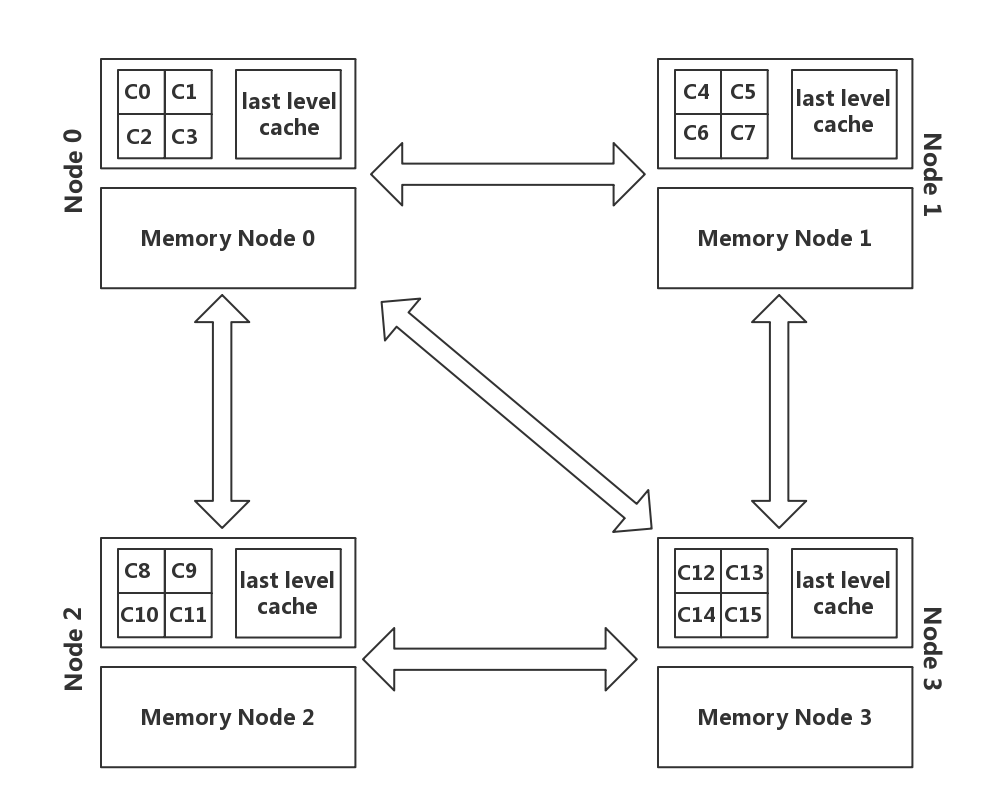
\includegraphics[width=5.0in]{NUMA.png}
	\caption{由四个四核处理器组成的NUMA系统}
	\label{Fig:numa}
\end{figure}
\section{NUMA架构及相关优化技术}

大型现代服务器通常由多个处理器节点组成,每个节点包含一个多核处理器和一块本地内存,其中本地内存上一般会有一个或多个内存控制器(memory controller)来处理来自本地节点或者其他节点上的核的内存访问请求,如图\ref{Fig:numa}所示。所有计算节点之间通过高速通信介质(interconnect)连接成单个缓存一致性系统,虽然物理内存被分割在了多个节点上,但是逻辑上物理地址空间仍然是全局共享的,也就是说所有核能够透明地访问所有节点上地物理内存。计算核心直接通过本地内存控制器来访问本地内存,而访问远程内存时则要通过节点间通信介质和远程内存的内存控制器。访问远程内存通常要比访问本地内存花费更多的时间,所以这些系统都具有非一致性内存访问时间(Non-Uniform Memory access, NUMA)的特征。再考虑到内存和缓存地层级化(memory hierarchy)设计,使得访存的非一致性更加显著。

显然要使应用程序在NUMA架构上获得最佳的性能,在放置应用程序的线程和内存数据时必须考虑系统资源的物理构成和分布,比如为了充分利用访存操作的局部性,将线程及其访问的数据放置在同一个node上来避免远程内存访问的巨大开销。由于NUMA架构的服务器的广泛应用,目前很多操作系统都针对NUMA因素做了通用的优化,比如很多Linux系统都提供了numactl用于查看和优化NUMA系统中的线程放置和内存管理。使用numactl中的numastat用户可以查看各个NUMA节点的内存分配和节点之间的内存访问状况,比如查看每个节点上运行的进程在该节点和其他节点上各申请了多少内存。通过设置numactl的参数用户可以限定应用只能运行在某些特定NUMA节点集合上或者限定该应用的内存只能分配在某些NUMA节点集合上。除此以外,numactl还可以设置更为复杂的内存分配核管理策略,比如是否使用巨页(huge page),内存是否交织(interleave)分布在所有或者某些节点上。

上述操作系统提供的的这些优化工具一方面是非常粗粒度的,另一方面要求用户必须事先了解所运行的程序的特征,而现实的应用特征是复杂多变的而且事先难以预测的,所以仅靠这些通用工具很难最大化应用的性能,进一步的优化必须监测和考虑应用程序本身的特征。Carrefour\cite{dashti2013traffic}在分析了大量应用程序的访存特征后,认为应该根据应用的内存访问特征来使用合适的内存放置和管理策略,如图\ref{Fig:carrefour}所示,Carrefour支持三种内存访问策略:
\begin{itemize}
\item  复制(replication),即将同一个页的拷贝放置在多个NUMA节点上,复制将热点数据的访问压力分摊到了多个内存控制器,同时避免了远程内存访问,但是必须保持多个复制页内容一致,类似于缓存一致性,代价非常高昂,所以一般只对读写比很高的页采用复制策略;
\item  交织(interleaving),即将内存页平均放置在所有节点上,从而平衡各个内存控制器和节点间通信介质的访问压力,操作系统提供的交织是全局性的,而Carrefour中的交织可以只对部分页使用,进行更细力度的内存管理;
\item 协同放置(co-locate),即将共享内存页的线程与其共享的内存页放置在同一个节点上,从而减少远程内存访问和缓存一致性操作。
\end{itemize}

\begin{figure}[t]
	\centering
	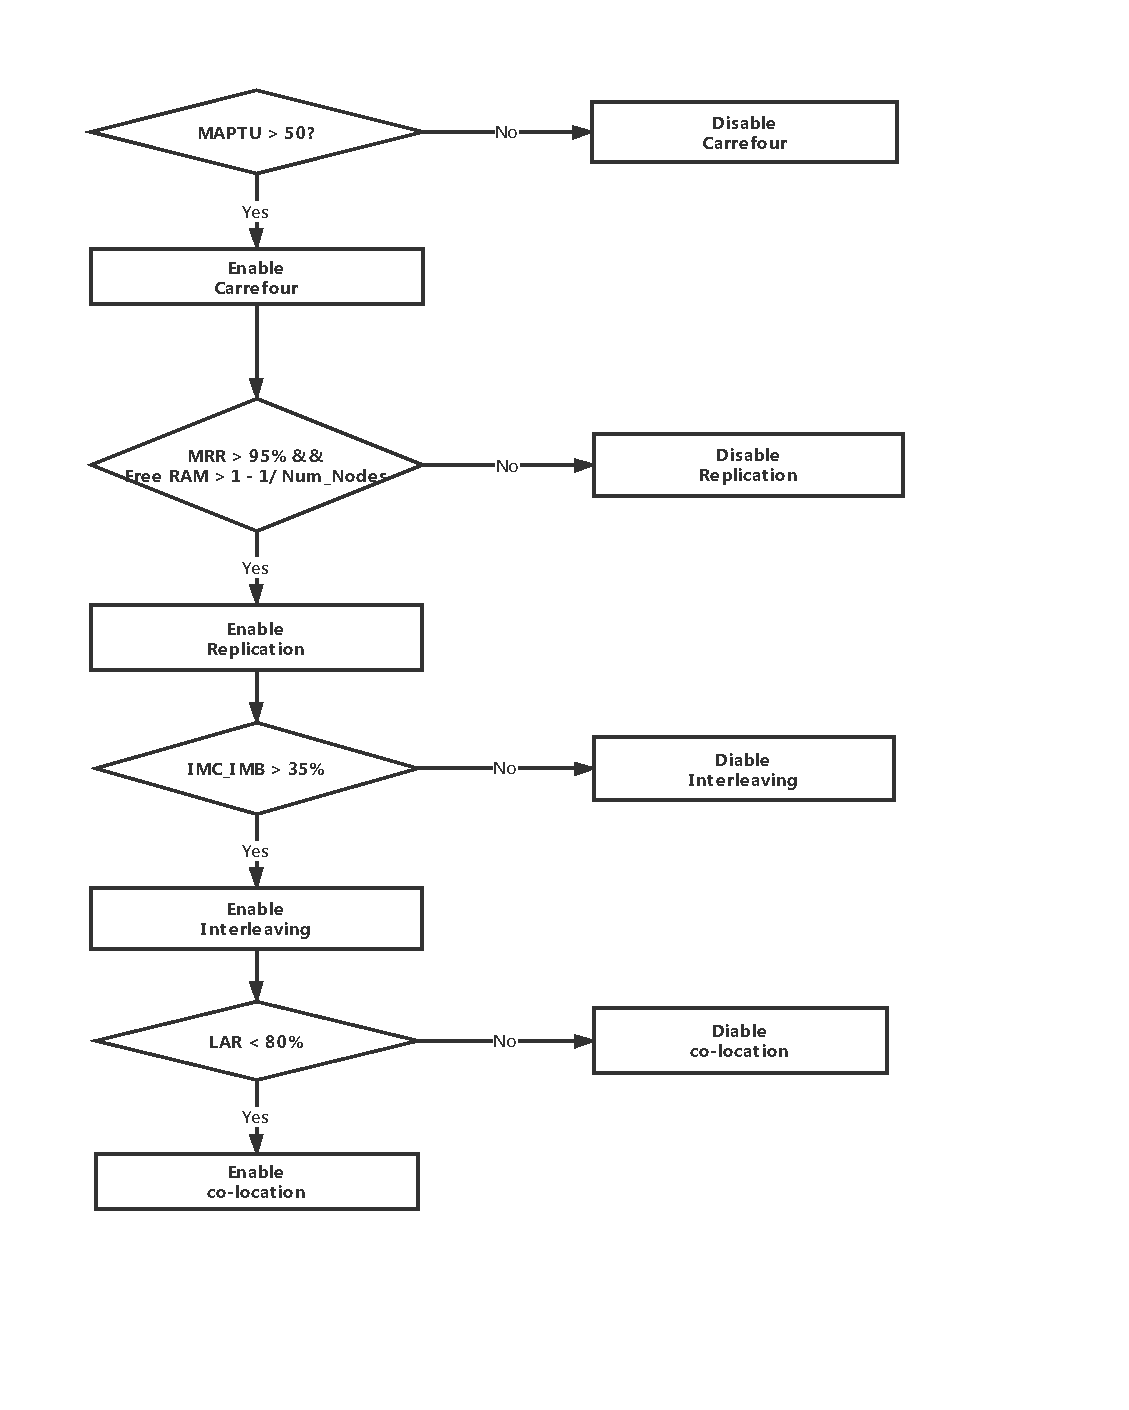
\includegraphics[width=4.2in]{Carrefour.pdf}
	\caption{Carrefour中的内存放置策略选择}
	\label{Fig:carrefour}
\end{figure}

\section{MCS锁与C-MCS锁}
\subsection{MCS锁}
MCS锁是一种基于单项链表的高性能、可扩展、公平的自旋锁,由John Mellor-Crummey和Michael Scott在1991年提出, 其名称来源于发明人的名字首字母。

MCS锁中包含一个指向队尾的指针tail,每个竞争者在队列中用一个记录(record)表示,其中每个记录包含一个指向后继节点的指针和一个表示当前是否可以进入关键区域的布尔变量。如图\ref{Fig:MCS}所示,每个线程请求锁时将自己记录中布尔变量设为false,然后使用compare\_and\_swap这个原子操作来完成以下操作将自身的记录加入队列:1)使tail指针指向自己的记录;2)将自己的记录连接在前驱节点(如果有的话)的后面。如果该线程有前驱节点,则它在自身记录的布尔变量上自旋直到其被前驱节点设为true然后进入关键区域,否则该线程将自己的布尔变量设为true直接进入关键区域。放锁时只需要将后继节点的记录中的布尔变量设为true然后断开于后继节点的链接即可,如果没有后继节点则将tail设为null。
\begin{figure}[t]
	\centering
	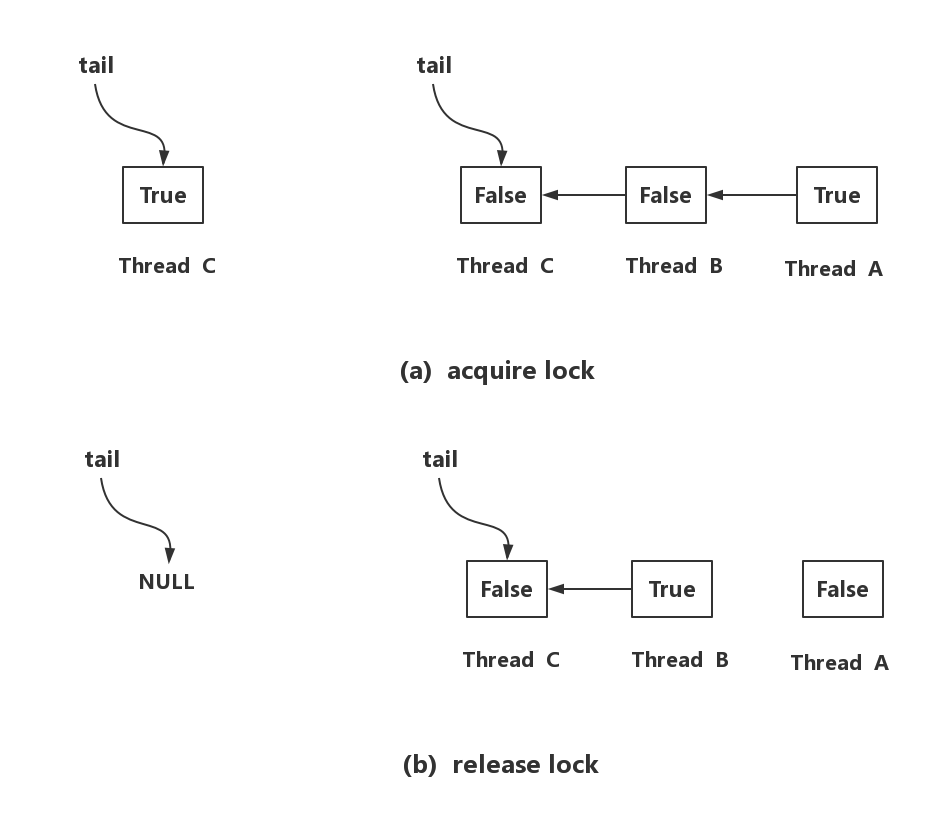
\includegraphics[width=5.6in]{MCS-lock.png}
	\caption{MCS锁拿放锁示例}
	\label{Fig:MCS}
\end{figure}

MCS的FIFO的公平性是通过显式存在的队列来维持的,其正确性由算法本身和compare\_and\_swap这个原子操作共同保证,每个线程只在本地标志变量上自旋并且只有自身和前驱节点对应的线程会访问该变量,这是MCS锁获得高性能和可扩展性的主要原因。

\subsection{C-MCS锁}
C-MCS锁是针对NUMA架构下内存及缓存访问的非一致性而对MCS锁做的适应性改进。它可以看作是一个两层的 MCS锁。如图\ref{Fig:CSTMCS}所示,该示例中展示了一个有9个线程的多线程应用,每个线程都差不多在同一个时刻竞争同一个锁(具体顺序如图(a)所示),其中线程T1到T5在节点0上而另外四个线程在节点1上,图a表示使用MCS锁时按照FIFO的顺序会有6次跨NUMA节点的锁传递(黄色表示跨节点锁传递),图b表示如果对锁的传递顺序加以合理调度则可以将跨节点的锁传递次数减为1,从而改善MCS锁在NUMA架构下的性能。a,b两图展示了C-MCS锁和MCS锁的本质差别,即C-MCS通过改变MCS锁的锁调度顺序,减少跨节点的锁传递频率,获得更好的性能。
\begin{figure}[t]
	\centering
	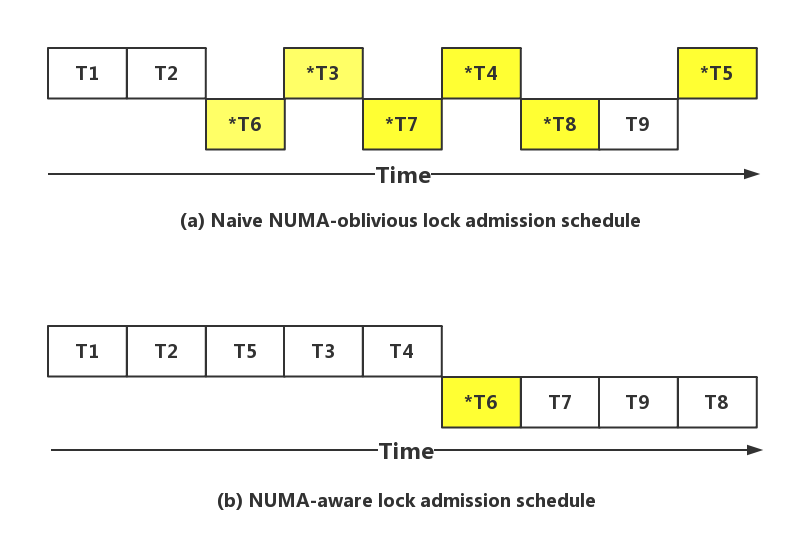
\includegraphics[width=5.0in]{CSTMCS.png}
	\caption{C-MCS锁示例}
	\label{Fig:CSTMCS}
\end{figure}
C-MCS的具体实现还是以MCS锁为基础,包含一个全局MCS锁和每个节点上的一个局部MCS锁。全局MCS锁在所有节点之间共享,它的主要作用时将竞争分隔在各个节点内;而每个局部MCS锁只在其所在的节点内的线程间共享。一个线程只有同时拿到全局MCS锁和其所在节点的局部MCS锁才可以进入关键区域。每个要执行关键区域的线程先竞争本地MCS锁,每个节点上第一个拿到本地MCS锁的线程继续竞争全局MCS,其他线程直接从第一个线程继承全局MCS锁。执行完关键区域的线程先释放本地MCS锁,如果锁在本地节点的传递次数超过了预先设定的上限或者本地节点上没有其他请求者的时候才会释放全局锁。所以C-MCS锁的传递顺序可以描述为,锁的持有者将其传给一个本地的最早请求者当且仅当以下两个条件同时满足:
\begin{itemize}
\item  本地节点当前至少有一个请求者;
\item  其所在本地节点的锁传递次数还未超过预先设定的threshold;
\end{itemize}
其中设置threshold是为了防止深层的不公平。

C-MCS锁在决定锁的调度顺序时考虑了等待队列中的线程和当前拿锁线程在NUMA拓扑上的相对位置,从而让减少了锁在NUMA节点之间的迁移频率,提高锁的总吞吐率。相反的,标准的MCS锁不能感知底层的NUMA因素,所以只能按照线程的到达时间即线程请求锁的时间来决定锁的传递顺序,所以在NUMA架构上会有性能损失,C-MCS锁放弃了MCS锁全局FIOF的锁传递顺序,只保证单个节点内的FIFO锁传递顺序,所以其高吞吐率的获取是以牺牲一定的短期公平性为代价的。

\section{线程调度与放置}
\subsection{NUMA架构下Linux线程调度}
作为资源管理的核心部分,操作系统的线程调度器的主要职责是保证准备好的线程被调度到可用的核上去。在Linux系统当前使用的调度算法CFS(Completely Fair Scheduling)\cite{lozi2016linux}是WFQ(Weighted Fair Queueing)调度算法的一种实现。在单CPU系统中,CFS的实现非常简单。为了实现公平调度,CFS定义了一个固定长度的时间间隔,在该间隔内系统中的每个线程至少运行一次,该间隔被按照线程的权重按比例分为若干个大小不一的时间片(time slice),每个线程的权重就是它的优先级。正在运行的线程会不断增加它的已运行时间(vruntime),当它的vruntime超过分配给其的时间片时,如果当前有其他可以运行的线程,那么正在运行的线程就会被抢占;另外当前运行的线程也可能被另一个被唤醒的vruntime更小的线程抢占。具体的实现中,线程被组织为一个用红黑树实现的运行队列(runqueue),如图\ref{Fig:CFS}所示在该运行队列中,每个线程按照其vruntime排序,当CPU需要找一个线程来运行的时候,红黑树中最左边的线程也就是vruntime最小的线程会被选择。

\begin{figure}[t]
	\centering
	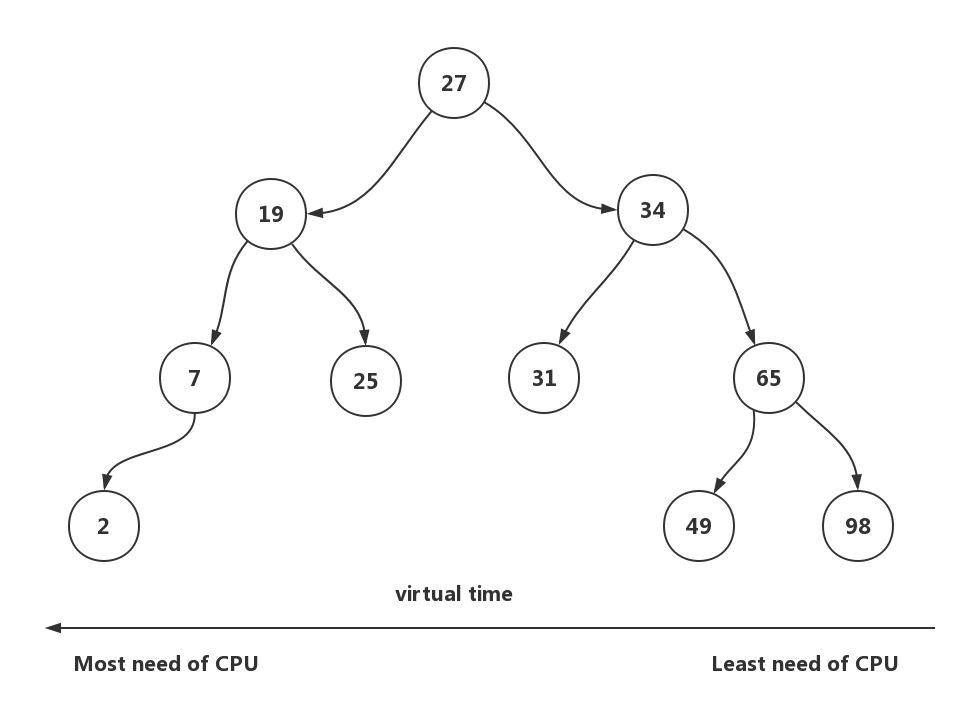
\includegraphics[width=5.0in]{CFS.png}
	\caption{CFS示例}
	\label{Fig:CFS}
\end{figure}

在NUMA架构下,由于缓存一致性和同步机制等的巨大代价及内存访问非一致性等原因的存在使得CFS的实现变得非常复杂。为了保持良好的可扩展性,CFS使用了per-core runqueue,即每个核一个运行队列,这样设计大的主要原因是进程切换(context switch)发生在关键路径上而每个核一个运行队列使得进程切换时只需要访问本地运行队列。但是为了使调度算法在使用了per-core runqueue时能够正确高效地运行,必须有额外的机制来保持运行队列的负载均衡。Linux CFS采用的方法是周期性地运行一个负载均衡算法来保持所有队列负载的大致均衡,具体实现中采用了层级化地策略(hierarchy strategy),所有核被逻辑上组织为一个层次结构,该层次结构的最底部是单个核,这些核在下一层及后面的层被如何分组是由它们对物理资源(内存,各级缓存)的共享拓扑决定的。每层的结构被称为一个调度域(scheduling domain),负载均衡算法按照自下而上的顺序在每个调度域内运行。将所有核组织成一个层次结构然后自下而上运行负载均衡算法相比直接在所有核之间通过线程迁移来调节负载的主要优势在于可以减少跨深层NUMA因素的线程迁移比例从而使得负载均衡算法的开销尽可能的小,这与层级锁的设计思路很相似。

现代操作系统的调度器在做线程调度时主要考虑因素有三点:1)通过线程在核之间的迁移来保证可运行的线程能被调度到可用的核上去;2)保证核之间负载的大致均衡;3)在NUMA架构下使负载均衡算法的代价尽可能大地小。这种调度算法非常适合相互之间没有关系的线程即不通过共享内存通信的线程,它能够避免线程之间对于节点层次的共享资源例如缓存、内存通道等的使用发生冲突(缓存失效等),它的前提假设是线程之间地通信非常少并且远不如节点层次地本地资源使用冲突重要。但是在锁集中并且存在大量线程间共享数据的多线程应用中,显然线程之间的通信是居于主导地位的,保证线程之间通信的高效的重要性要高过线程对资源的独享重要性\cite{dice2015lock},所以操作系统通用的调度器不能很好的满足这类场景的需求。另外考虑到层级锁中通过挖掘线程之间的亲和性来做锁调度,而通用的调度器将相关的线程分散在所有节点的可用核上使得层级锁可以挖掘的线程间的亲和性非常有限。

综上来看,通用的调度器并不适合NUMA架构下锁集中的多线程应用尤其是使用层级锁多线程的应用,为了使这些应用获得更好的性能,必须有定制化的考虑应用具体特征的线程调度/放置方法,也就是说应该使用定制化的调度器或者让应用程序来做自身的线程调度/放置。


\subsection{NUMA架构下针对锁的线程调度优化}
在NUMA架构下,操作系统的通用调度器很容易造成锁在NUMA节点之间的频繁迁移进而导致其性能下降,所以出现了很多定制化的线程放置/迁移策略,比如最朴素的做法是将请求锁的线程迁移到当前持锁的线程锁在的节点,即将线程迁移到包含锁及其保护的数据的缓存而不是相反,然而这种简单的迁移存在两个问题:1)线程迁移次数不可控;2)容易导致负载不均衡,最终的结果可能是得不偿失。shuffling\cite{pusukuri2014shuffling}是一种能够兼顾负载均衡和迁移代价的适合锁集中的应用的线程放置/迁移策略。shuffling通过将到达时间(lock arrival time)差不多的线程放置在相同的节点上来避免锁在节点间随意迁移,具体做法如图\ref{algo:shuffling}所示,shuffling周期性地收集各个线程的到达时间;然后按照到达时间将所有线程排序分组,到达时间相似的线程被分到相同的组里,每组的大小等于每个节点上的计算核心数;最后通过迁移某些线程将分好的每个线程组映射到NUMA节点上去。相比简单的线程迁移,shuffling保证了负载均衡并且可以很好地控制线程的迁移。

\begin{algorithm}
% \begin{algorithm}[H] % 强制定位
\caption{Shuffling框架}
\label{algo:shuffling}
\begin{algorithmic}[1] %每行显示行号
\Require N:Number of threads, C:Number of Sockets % 输入
\Repeat
\State {\bf i. Monitor Threads} -- sample lock times of N threads
\If{\emph{lock times exceed threshold}}
    \State {\bf ii. Form Thread Groups} -- sort threads according to lock times and divide them into C groups
    \State {\bf iii. Perform Shuffling} -- shuffle threads to establish newly computed thread groups
\EndIf
\Until{application terminates}
\end{algorithmic}
\end{algorithm}

\subsection{现有针对层级锁的线程放置策略}
在层级锁中,上述将请求锁线程迁移到当前持锁线程锁在NUMA节点上显然是没有必要的,因为层级锁并不是按原有锁的传递顺序来传递的。层级锁通过利用线程之间的亲和性来调度锁进而减少锁在节点间的迁移,所以对于层级锁来说最自然最高效的线程放置策略就是在保持负载均衡的前提下将线程尽可能地放得紧凑,所以大多数地层级锁将每个线程绑定到一个专用地核上,只有当前地节点上没有可用的核时才会将新的线程放置在一个新的节点上。此外,也有的层级锁出于测试锁的某些方面的表现等其他目的而将线程平均放置在所有节点上。我们在下一章中会对这两种线程放置策略进行进一步地分析和说明。

\section{锁替换技术}
由于Pthread(POSIX Threads)线程库具有很好的平台可移植性,所以很多历史遗留的多线程应用,比如Memcached,都采用了Pthread线程模型,相应地Pthread mutex也就成了这些应用中最常用的锁。为了在这些应用中测试和使用其他锁并且省去冗长且容易出错的手动替换的麻烦,Hugo Guiroux\cite{guiroux2016multicore}开发了LiTL(Library for Transparent Lock interposition)。

LiTL是一个Linux/x86平台下可以在运行时将基于Pthread mutex的应用中的Pthread mutex替换为其他锁的库。为了实现锁替换,LiTL使用一个可扩展的并发哈希表(CLHT\cite{david2015asynchronized})维护了一个标准Pthread锁(pthread\_mutex\_t)实例和其他用来替换Pthread mutex的锁实例(比如MCS锁)的映射,也就是说LiTL必须追踪Pthread mutex从pthread\_mutex\_init()到pthread\_mutex\_destroy()的整个生命周期,并且在该生命周期中,每次pthread\_mutex\_lock()都会必须触发一个在上述映射中查找对应其他锁实例的查找操作。此外,某些锁的lock/unlock接口除了锁变量本身以外还需要其他参数,比如在MCS锁中该额外参数对应每个线程的记录(record),对于这些锁,LiTL还在映射中为每个锁实例每个线程维护了一个额外的结构体来表示这些额外参数。

LiTL使用LD\_PRELOAD来拦截基于Pthread mutex的应用中类似pthread\_mutex\_*这样的函数调用,然后查询CLHT,找到对应的映射锁实例,调用对应的函数。LD\_PRELOAD利用了Linux系统中动态链接器(dynamic linker)提供的功能来使用户可以指定动态链接器在加强其他共享库之前绑定某个库的符号(symbol),LiTL提供了与Pthread库相同的外部接口,所以替换Pthread mutex的锁对应的库通过LD\_PRELOAD在应用运行时优先加载后,所有Pthread mutex相关的调用最终都会被拦截到LiTL提供的库中。

\section{本章小结}
本章主要对本文研究所基于的平台和相关技术进行了说明,包括NUMA架构的特性及相关的优化技术,MCS锁、C-MCS锁的实现及特性,Linux系统下的通用调度器的特性及其局限性,还有针对锁集中的应用的一些线程放置策略及其优化,以及锁替换技术等。这些相关的研究和技术一方面是本文研究的基石,另一方面也为本文的研究提供了很多有益的启发和借鉴,比如本文的提出的线程放置框架的混合特性与Carrefour的混合内存放置策略相似,为了保证长期公平性而使用的shift机制与Malthusian锁的shift机制的做法和目的都很相似,而竞争感知的特性则是借鉴了AHMCS锁的竞争感知。
%# -*- coding: utf-8-unix -*-
%%==================================================
%% chapter02.tex for SJTU Master Thesis
%% based on CASthesis
%% modified by wei.jianwen@gmail.com
%% Encoding: UTF-8
%%==================================================

\chapter{建模与分析}
\label{chap:example}
我们首先定义锁K的吞吐率为单位时间内K在竞争K的线程间的的平均传递次数,定义单个线程T的吞吐率为单位时间内K在T上的平均传递次数。此外,本文中锁K的长期公平性指的是长远来看,各个线程的拿锁次数之间的差异程度,可以用变异系数来衡量,变异系数越小,长期公平性越好。线程放置策略决定了线程在NUMA节点之间的分布,进而影响锁在NUMA架构机器上的吞吐率。而对于层级锁来说,由于其本地偏好的锁传递规则的影响,线程放置策略还会影响其长期公平性。本章以两层的MCS锁即C-MCS锁为例,首先通过实验验证紧凑策略和平均策略在基于队列的层级锁的吞吐率和长期公平性方面的表现,然后建模分析线程放置策略影响吞吐率和长期公平性的根本因素,进而得出线程放置策略优化应遵循的原则和面临的挑战。

\section{实验验证}
我们的实验跑在Intel Xeon E5上,该机器由四个NUMA节点组成,每个节点上包含八个计算核心。实验的benchmark取自libslock中的stress\_one,实验中用到的锁是C-MCS锁,该锁是一个两层的MCS锁,包括一个全局MCS锁和每个节点上的本地MCS锁。实验中stress\_one被配置为使用12个线程,每个线程重复以下操作:拿锁,写一定大小的缓存,放锁,暂停一段时间。该实验中我们用暂停时间的长短来控制锁的竞争强度的大小,暂停时间越短,锁的竞争越激烈,实验中用到了两个暂停
时\begin{table}[!hpb]
  \centering
  \bicaption[吞吐率对照]
    {吞吐率(acquisitions/s)}
    {Aggregate Throughput}
  \label{tab:aggregate}
  \begin{tabular}{@{}llr@{}} \toprule
    暂停时长 & 紧凑放置 & 平均放置\\ \midrule
    5000 cycles & 4574093 & 3101512 \\
    500  cycles & 4401877 & 4273903\\
  \end{tabular}
\end{table}
间:500时钟周期和5000时钟周期。图\ref{Fig:compact}和图\ref{Fig:even}分别展示了该实验在紧凑和平均(AHMCS中将平均放置到所有节点上,而本实验中也是平均放置,但为了获得更高吞吐率,我们是只使用了两个节点)两种放置策略下单个线程的吞吐率,其中在平均放置策略中我们只是用了4个NUMA节点中的两个节点。上述两张实验图中每个长条代表单个线程的吞吐率,而不同颜色表示不同的竞争强度。表\ref{tab:aggregate}和表\ref{tab:CV}分别显示了不同配置下的吞吐率及变异系数。

\begin{table}[!hpb]
  \centering
  \bicaption[变异系数对照]
    {变异系数}
    {Coefficient of Variance}
  \label{tab:CV}
  \begin{tabular}{@{}llr@{}} \toprule
    暂停时长 & 紧凑放置 & 平均放置\\ \midrule
    5000 cycles & 64.174778\% & 1.939154\%\\
    500  cycles & 35.315475\% & 0.036318\%\\
  \end{tabular}
\end{table}

从表\ref{tab:aggregate}中可以看出,两种竞争强度下的最高吞吐率比较接近,即增加单个线程的锁请求频率并未增加吞吐率,所以上述两种竞争强度下C-MCS锁都已经达到了饱和。在锁达到饱和并且关键区域执行时间不变的情况下,影响吞吐率的最主要的因素将是锁传递的平均时延大小,而在NUMA架构下影响锁传递平均时延大小的主要是锁在NUMA节点之间传递的频率。

结合图\ref{Fig:compact}、表\ref{tab:aggregate}和表\ref{tab:CV}可以看出紧凑放置能够尽可能地保证层级锁的高吞吐率,但是吞吐率在线程之间地分布是严重不均衡的,同一个NUMA节点上的线程吞吐率基本相同,不同NUMA节点上地线程之间吞吐率差别可以达到十几倍,而且实验中的两种竞争强度下受益的线程集合正好相反。结合图\ref{Fig:even}、表\ref{tab:aggregate}和表\ref{tab:CV}可以看出平均放置能够保证层级锁的长期公平性,单个线程的吞吐率之间没有明显的差异,但是即使在总的竞争已经饱和而且在平均放置的基础上使线程放置地尽可能地紧凑的情况下,如果竞争并不是很高其总的吞吐率相比紧凑放置还是有明显地损失,实验中其总吞吐率损失多大32.2\%。

\begin{figure}[t]
	\centering
	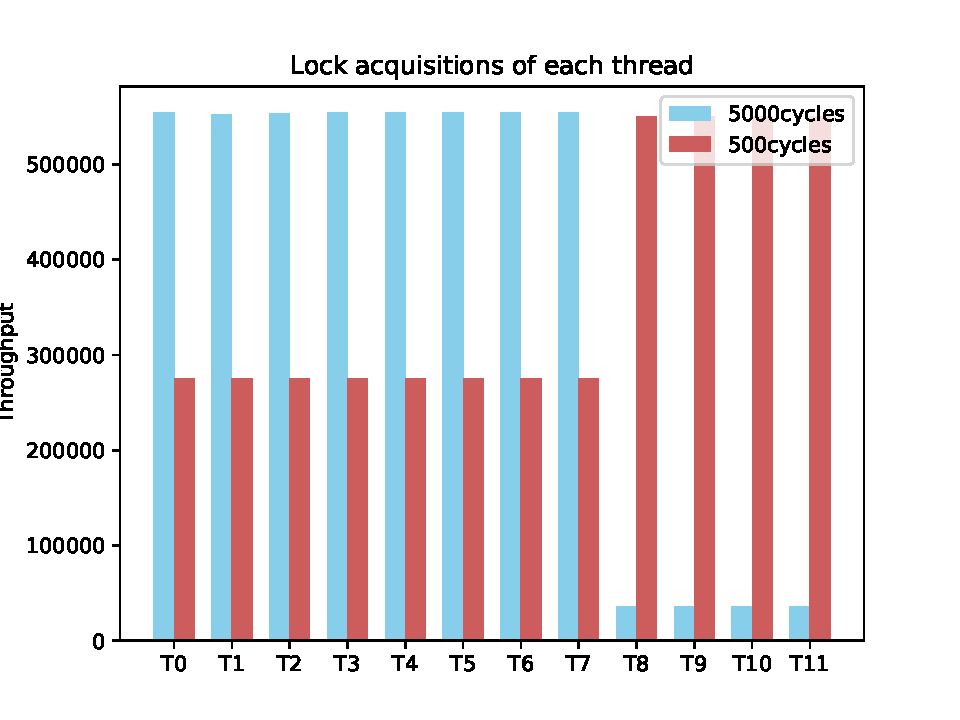
\includegraphics[width=5.6in]{compact.pdf}
	\caption{紧凑放置:单个线程的吞吐率}
	\label{Fig:compact}
\end{figure}

\begin{figure}[t]
	\centering
	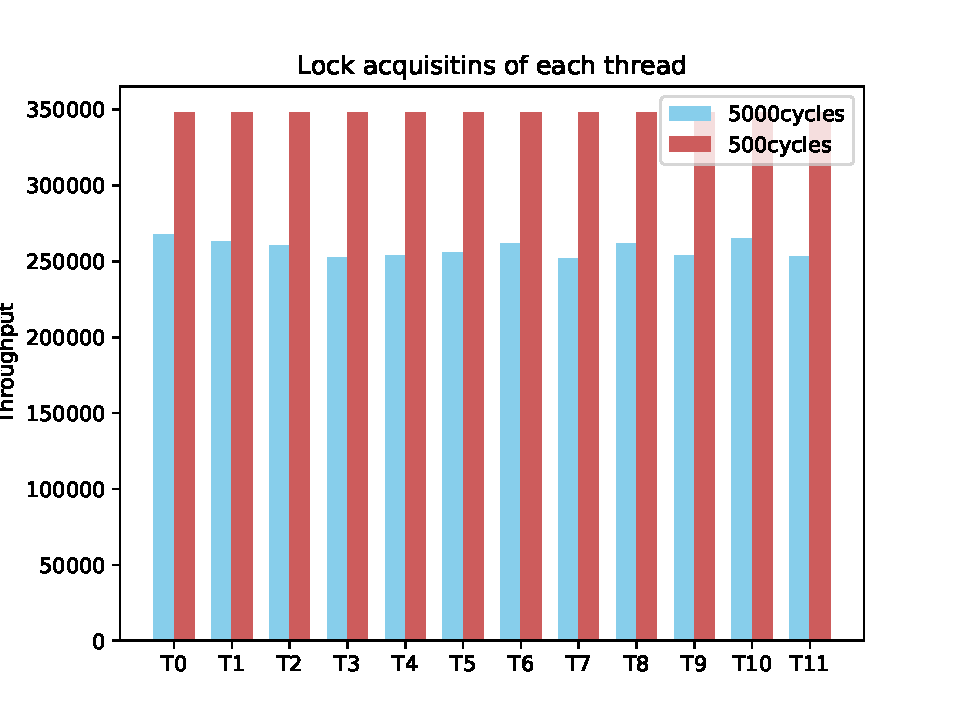
\includegraphics[width=5.6in]{even.pdf}
	\caption{平均放置:单个线程的吞吐率}
	\label{Fig:even}
\end{figure}

\section{建模}
本小节中我们以C-MCS锁为例,通过建模从微观角度分析线程放置策略中影响基于队列的层级锁的总吞吐率和长期公平性的关键因素。

\begin{figure}[t]
	\centering
	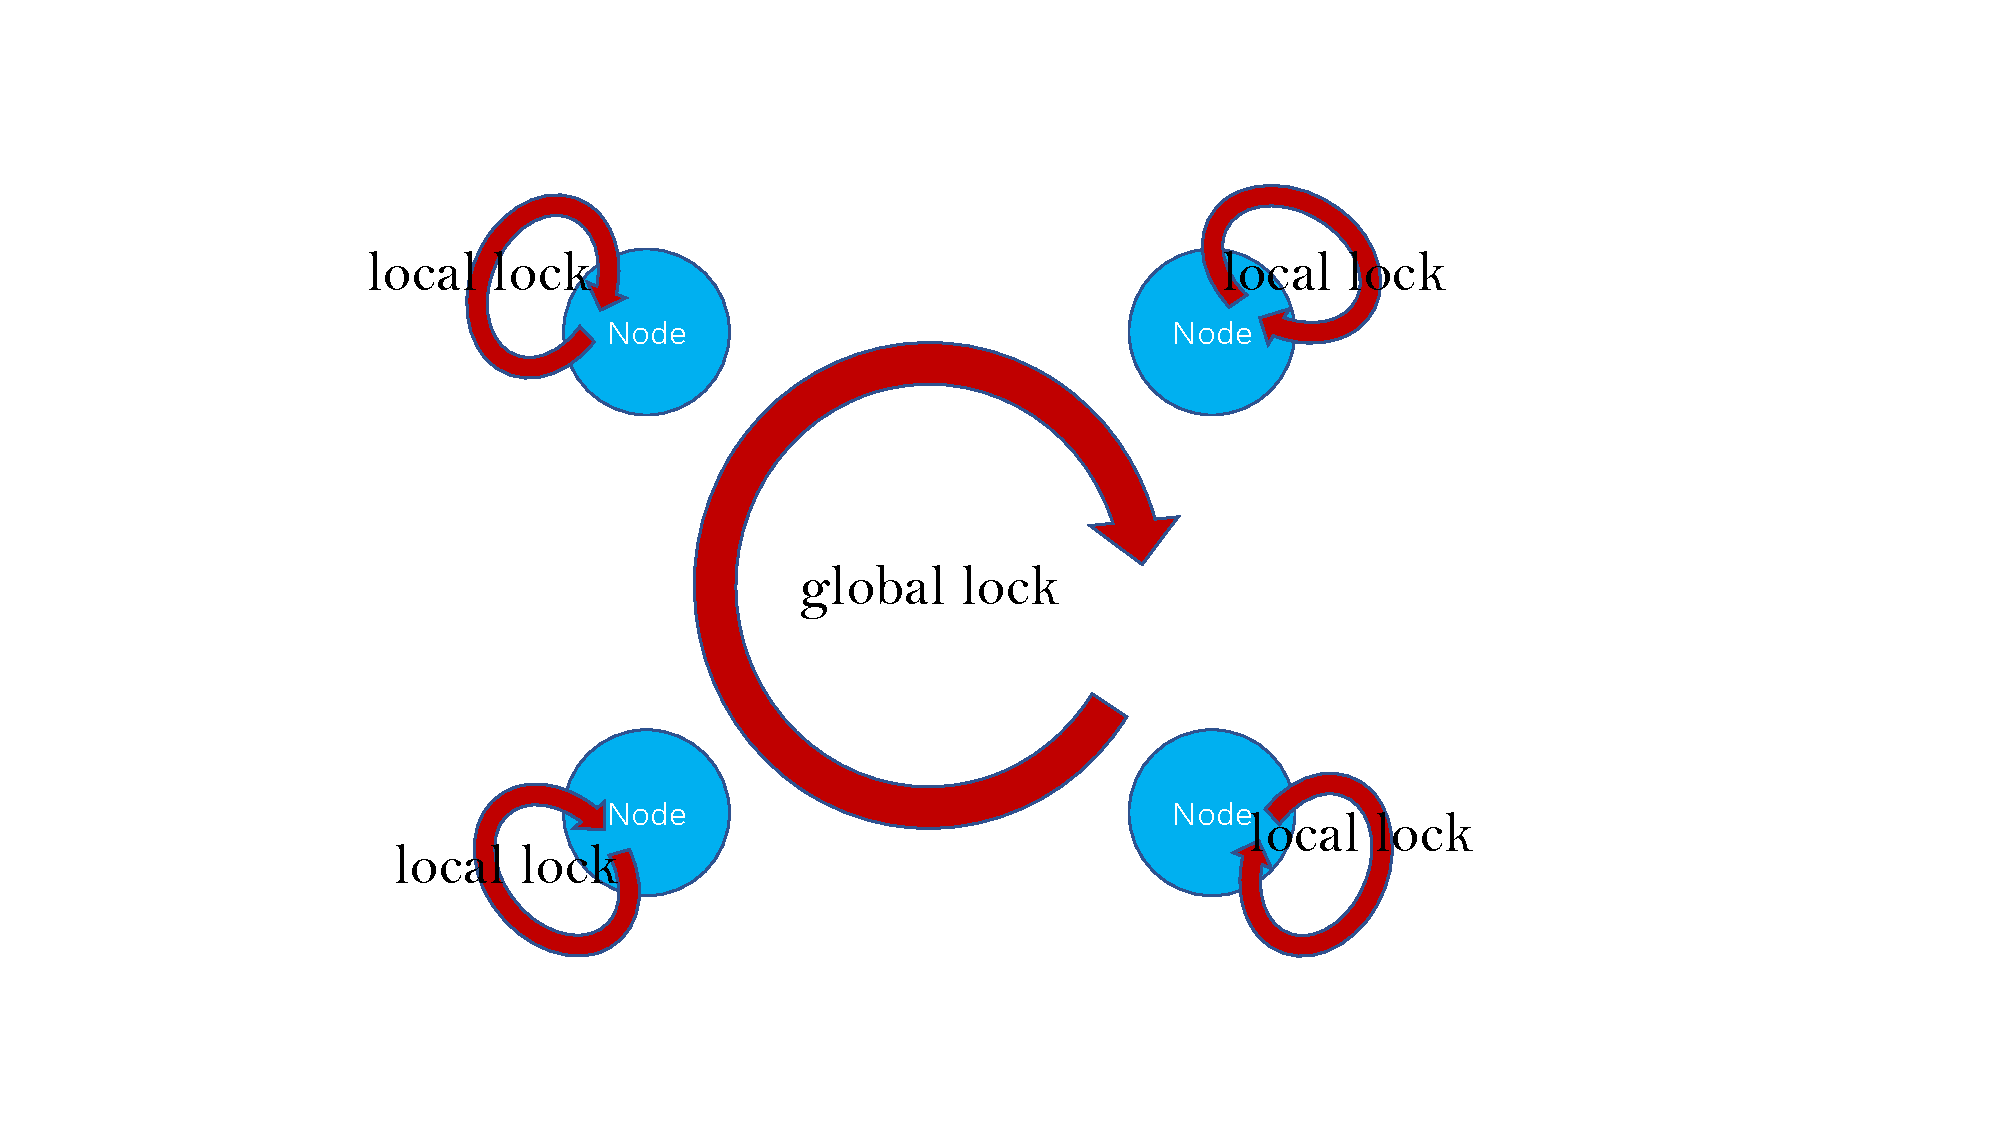
\includegraphics[width=5.6in]{circulation.pdf}
	\caption{C-MCS锁中的一个循环}
	\label{Fig:circulation}
\end{figure}

因为层级锁主要用于竞争线程较多竞争较激烈的场景,所以以下建模分析基于层级锁的竞争较为激烈至少已经饱和的假设。C-MCS锁中用到的全局锁和本地锁都是MCS锁,而MCS锁按照先进先出(FIFO,first in first out)的顺序在线程之间传递,所以我们可以认为全局MCS锁在相关NUMA节点之间按照round-robin的方式传递;对于某个特定节点上的线程来说,当第一个请求者代表该节点拿到全局锁时,对应的本地MCS锁在该节点上运行的所有相关节点之间也按round-Robin的方式传递,直到最后一个请求者释放全局锁(当前节点没有后续请求者)或者某个请求者被强制释放全局锁(当前节点上的传递次数达到threshold),如图\ref{Fig:circulation}所示。为了说明的方便,我们将全局MCS锁在所有相关节点之间传递一次的时间间隔定义为一个循环(circulation),并且以一个循环为单位来评估吞吐率和长期公平性。


我们用N表示竞争锁的线程数,这些线程分布在S个节点上,大小为S数组Count中每个元素Count[i]表示节点i上放置的线程数,则有约束:
\begin{equation}\label{Eq:threads}
  \sum_{i=1}^{S} Count[i] = N
\end{equation}
\begin{equation}\label{Eq:non-zero}
  Count[i] > 0 \quad for\;each\;  i\; in\; 1\;to\;S
\end{equation}
其中S及Count数组中每个元素的大小都是由线程放置策略决定的,只要满足上述约束即可。我们用大小为N的数组Acquisitions中每个元素Acquisitions[i]表示线程i在一个循环内的拿锁次数,用interl表示跨节点的锁传递时延,用intral表示同一节点内的锁传递时延,则一个循环的总时间可以表示为
\begin{equation}\label{Eq:duration}
 Duration=\sum_{i=1}^{N} Acquisitions[i] * intral + S * (interl - intral)
\end{equation}
一个循环内总的锁传递次数可以表示为
\begin{equation}\label{Eq:totalacqui}
  TotalAcquisitions=\sum_{i=1}^{N} Acquisitions[i]
\end{equation}
进而吞吐率可以表示为
\begin{equation}\label{Eq:total-thrpt}
 Throughput=\frac{TotalAcquisitions}{Duration}
\end{equation}
一个循环内每个线程的平均拿锁次数为
\begin{equation}\label{Eq:AVG}
  \mu = \frac{TotalAcquisitions}{N}
\end{equation}
标准差为
\begin{equation}\label{Eq:SD}
  \sigma=\sqrt{\frac{\sum_{i=1}^N(Acquisitions[i]-\mu)^2}{N}}
\end{equation}
而变异系数可以表示为
\begin{equation}\label{Eq:CV}
 c_v=\frac{\sigma}{\mu}
\end{equation}

由式\ref{Eq:duration}到式\ref{Eq:total-thrpt}可知$\sum_{i=1}^{N} Acquisitions[i]$越大,即一个循环内总的锁传递次数越多,吞吐率越高;而由式\ref{Eq:totalacqui}、式\ref{Eq:AVG}和式\ref{Eq:CV}可知,Acquisitions中N个元素越接近,即N个线程的拿锁次数之间的差异越小,变异系数越小,长期公平性越好。故吞吐率和变异系数都与一个循环内每个线程的拿锁次数有关,所以以下我们按照C-MCS锁的传递规则对一个循环内每个元素的拿锁次数Acquisitions[i]进行建模。

对于只有一个线程的应用来说,其任何时刻在执行关键区域的概率可以表述为:
\begin{equation}\label{Eq:pro}
     P_{cs} = CS / (NCS + CS)
\end{equation}
其中CS和NCS分别代表关键区域和非关键区域的长度。那么对一个包含T个请求同一个锁的线程的应用来说,其任何时刻在执行或者等待执行关键区域的线程数的期望值为:
\begin{equation}\label{Eq:expectation}
     E_{cs} = T * P_{cs}
\end{equation}
\emph{Ecs}由应用中锁的竞争者的数量和单个竞争者请求锁的频率计算而来,可以用来表示和评估应用中的锁的总体竞争强度,Ecs越大意味着锁被请求的越频繁,即锁的竞争越激烈。当\emph{Ecs}的值为1时,锁被持续持有并且所有线程无需等待就能在请求锁的时候就拿到锁,如图\ref{Fig:saturation}所示,此时的线程数即为该锁当前的饱和点\cite{dice2017malthusian}。由式\ref{Eq:expectation}可得饱和点的值可以表示如下
\begin{equation}\label{Eq:sat}
     Sat = (NCS + CS) / CS
\end{equation}

\begin{figure}[t]
	\centering
	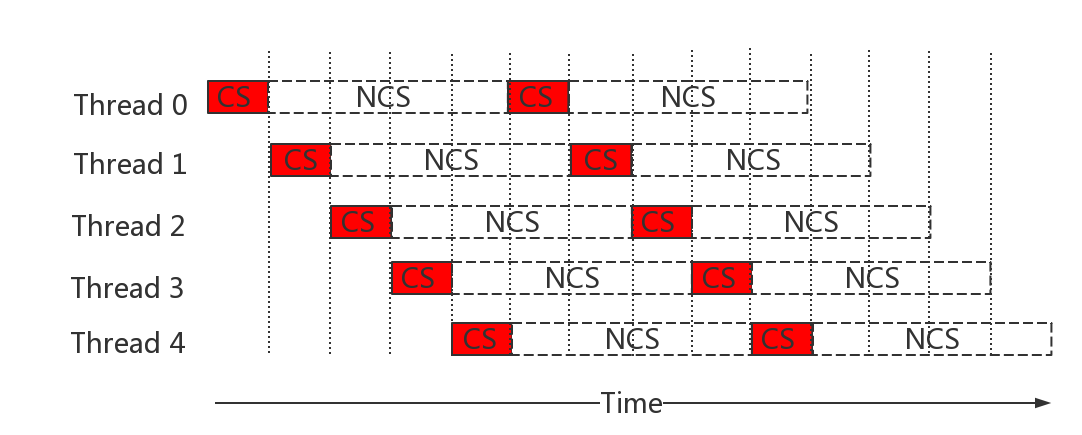
\includegraphics[width=5.6in]{saturation.png}
	\caption{饱和点,该图示中饱和点为5}
	\label{Fig:saturation}
\end{figure}

现在考虑C-MCS锁的传递规则,在每一个循环中,如果NUMA节点k上的线程数Count[k]大于等于饱和点Sat,则节点k上的任何一个线程在放锁时总是至少有一个线程在等待锁,所以锁会在该节点上一直传递直到节点k上总的传递次数达到预先设定的上限threshold;否则节点k上的最后一个线程放锁后其他线程还在执行非关键区域,故一个循环内锁在该节点上的传递次数为Count[k]。即
\begin{equation}\label{Eq:localtrans}
node\_acquisitions =
\begin{cases}
Count[k] &\text{Count[k] < Sat}\\
threshold &\text{otherwise}
\end{cases}
\end{equation}
因为每个节点上的本地MCS锁是完全公平的,所以我们可以认为同一个节点上的每个线程的在一个循环内的拿锁次数相等,即节点k上每个线程i在一个循环里边的拿锁次数为
\begin{equation}\label{Eq:per}
Acquisitions[i] =
\begin{cases}
1 &\text{Count[k] < Sat}\\
\frac{threshold}{Count[k]} &\text{otherwise}
\end{cases}
\end{equation}
一般情况下为了获取更高的吞吐率,threshold通常被设为Count[k]的若干倍,所以每个节点上放置的线程能否使该节点上的本地锁饱和对于该节点上的每个线程在一个循环内的拿锁次数影响很大。

\section{模型分析}
基于上述建模,我们可以得出下述结论:
\begin{itemize}
    \item 吞吐率由一个循环内总的锁传递次数决定,一个循环内总的所传递次数越多,吞吐率越高;
    \item 长期公平性由一个循环内各个线程拿锁次数之间的离散程度决定,各个线程拿锁次数越接近,长期公平性越好;
    \item 一个循环内同一个节点内的线程的拿锁次数相等;
    \item 一个循环内两个不同节点l和m上的线程的拿锁次数是否相等由Count[l]和Count[m]是否相等决定的;
    \item 节点k上放置的线程数Count[k]与饱和点Sat的关系决定了一个循环内节点k上每个线程的拿锁次数是1还是$\frac{threshold}{Count[k]}$,并且一般情况下threshold被设置为Count[k]的若干倍。
\end{itemize}
所以在基于队列的层级锁中获取尽可能高吞吐率的一个充分条件是保证尽可能多的节点上放置的线程数大于等于饱和点Sat;而保证长期公平性的一个充分条件是使所有节点上放置的线程数相等。本章开头的实验中紧凑放置在竞争较小时(此时Sat较大)相比平均放置能够获得更高吞吐率的原因就在于,此时紧凑放置至少保证了一个节点上放置的线程数大于等于饱和点,而平均放置中两个节点上放置的线程数都小于饱和点;紧凑放置在两种竞争强度下都不能保证长期公平性的原因则在于两个节点上放置的线程数不相等。

\begin{figure}[t]
	\centering
	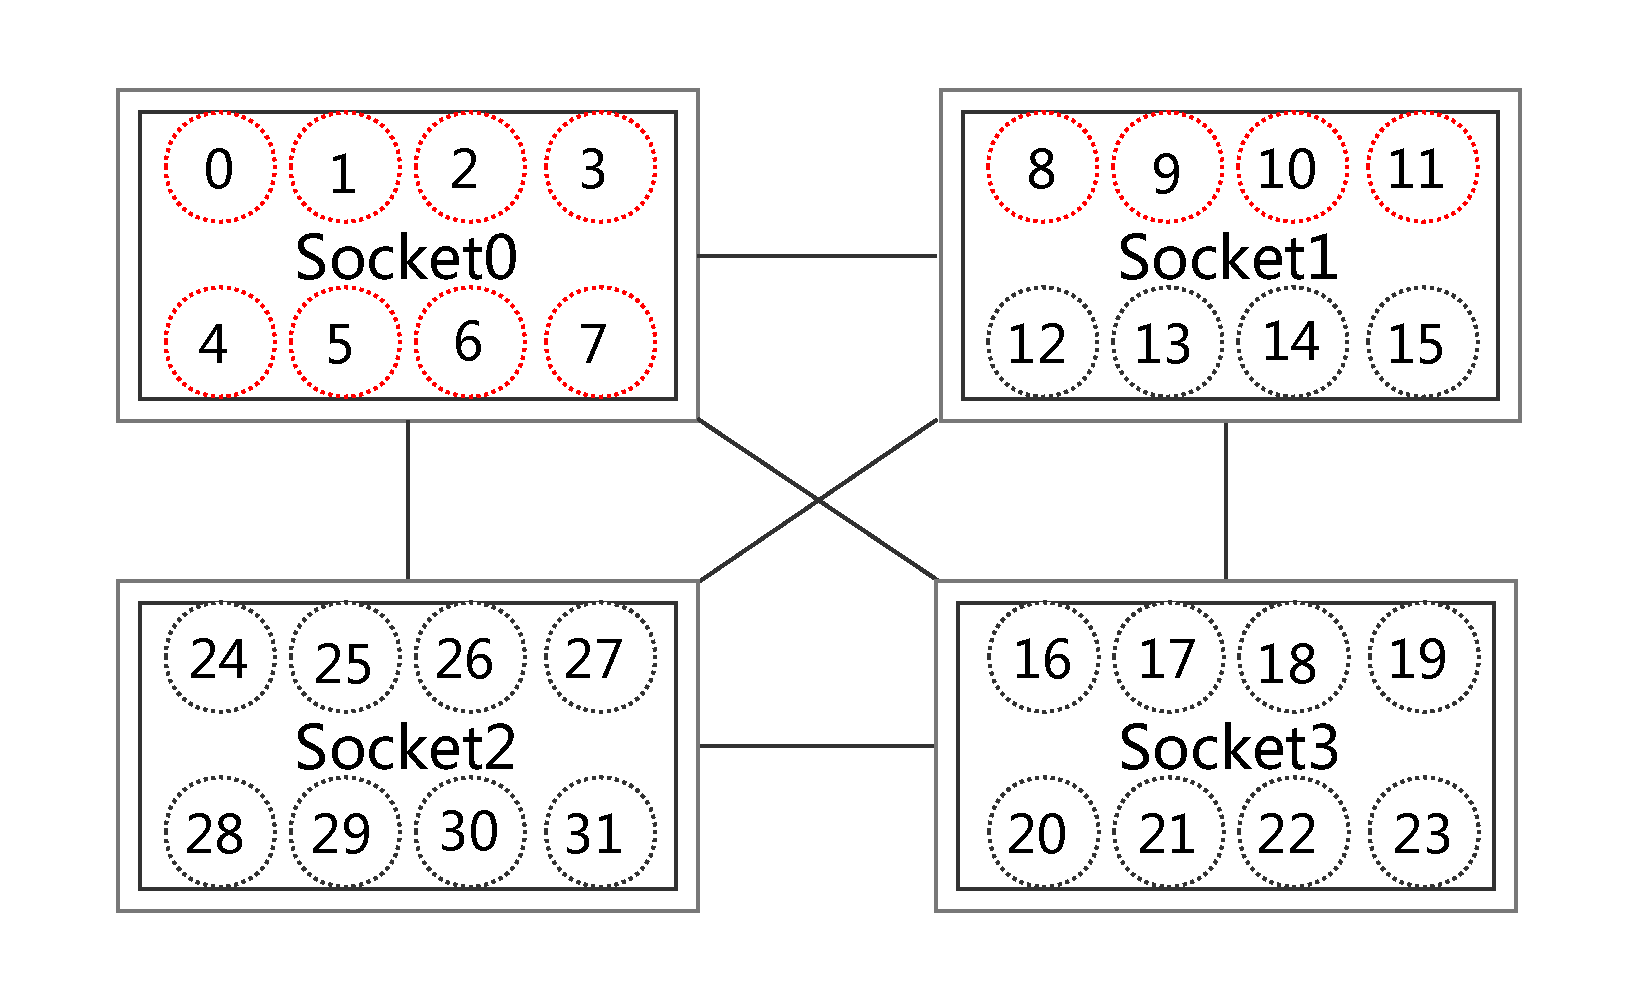
\includegraphics[width=5.6in]{symmetric.pdf}
	\caption{线程等价类}
	\label{Fig:symmetric}
\end{figure}

为了进一步说明线程放置对基于队列的锁的长期公平性的影响,我们定义两个线程之间的关系为对称(symmetric)如果不管锁的竞争强度如何变化,这两个线程理论上长期的拿锁次数差距为0。由上述建模及分析可知,运行在同一个NUMA节点上的任何两个线程之间是对称的;而对于运行在两个不同节点上的线程来说,当这两个节点上运行的线程数量相等时,这两个线程是对称的。显然,对称关系是一种等价关系,因此所有竞争同一个层级锁的线程可以按照其在NUMA节点上的分布来被分为若干等价类。例如,图\ref{Fig:symmetric}中的20个线程可以分为两个等价类,其中节点0上的8个线程和节点3上的8个线程属于同一个等价类,剩下的4个线程属于另一个等价类。所以我们也可以说保证基于队列的层级锁的长期公平性的一个充分条件是使所有线程按照对称关系属于同一个等价类。

\section{挑战分析}
从上述建模和分析可以看出从线程放置的角度保证基于队列的层级锁的吞吐率和长期公平性两者之一是非常简单直接的,但是同时保证两者则要面临以下限制挑战:
\begin{enumerate}
  \item 节点k上可以放置的线程数Count[k]应该小于等于节点k上的计算核心数,否则可能会产生锁的持有者或等待着被抢占的问题;
  \item 应用中的线程数和饱和点都可能随着上层的业务需求和下层的硬件资源状况变化,简单单一的线程放置策略只能在某些情况下同时保证高吞吐量和长期公平性;
  \item 受制于单个节点上所能放置的线程数,保证每个节点上的放置的线程数相等和保证尽可能多的节点上放置的线程数大于等于饱和点这两个目标有时候很难同时达到。
\end{enumerate}

在公有云等很多共享资源的场景下,资源的高效利用和资源在用户间的公平分配对于其的成功同等重要;这些应用场景同时也因为价格、时段等因素的影响,资源的需求变化很大,再加上多种应用共享底层硬件资源带来的影响,使得共享资源的竞争很难预测和控制。这些都对共享资源的分配和利用提出了新的挑战,从本章的分析可以看出线程放置对于使用层级锁的应用中的共享资源的利用和其在线程间的分配有很大影响。而现有的简单单一的线程放置策略不能满足应用在各种复杂多变的需求下对层级锁吞吐率和长期公平性的需求,我们需要额外的技术和更复杂更合理更细力度的线程放置策略来应对这些挑战。

\section{本章小结}
在这一章中,我们首先通过实验展示了现有基于队列的层级锁中线程放置策略在吞吐率和长期公平性方面的存在的缺陷,然后通过对吞吐率和长期公平性建模分析出了决定基于队列的层级锁的吞吐率和长期公平性的关键因素,最后在此基础山得出了基于队列的层级锁中线程放置策略所面临的挑战,从而为后续说明竞争感知的混合线程放置策略做好了理论基础。
%# -*- coding: utf-8-unix -*-
\chapter{设计与实现}
\label{chap:faq}
基于上一章的建模和分析我们发现很多场景下基于队列的层级锁中性能和长期公平性对线程的放置是很难同时满足甚至相互冲突的,再加上应用中锁的竞争强度的复杂多变,简单单一的线程放置策略不可能在竞争强度变化的情况下总是同时保证基于队列的层级锁的性能和长期公平性。针对上述挑战我们提出了一种新的竞争感知的混合线程放置框架CAH。本章我们将详细介绍CAH的设计与实现,我们先给出CAH的一个综述,再就设计与实现中的某些重要的方面做具体的解释。

\section{综述}
CAH是一种竞争感知的混合线程放置框架,它能用适应不同的竞争强度,能用尽可能小的额外代价同时保证高吞吐率和长期公平性。其中高吞吐率通过在每个相关NUMA节点上放置足够多的线程从而减少锁在节点之间的迁移频率来达到;长期公平性通过将线程平均放置在相关节点上或者定期交换不同等价类中的线程从而抹平线程间的吞吐率差异来保证。

\subsection{改进现有放置策略}
CAH针对原有平均放置和紧凑放置的缺陷对其分别做了改进。AHMCS的作者为了测试其对于竞争状况变化的响应速度而采用的平均放置是一种稀疏(sparse)的平均放置,即将线程平均放置在所有可用的NUMA节点上,由于线程分布过于稀疏导致层级锁不能充分地挖掘和利用线程之间的亲和性,所以原有平均放置通常不能达到高吞吐率。本文中我们为了获取更高的吞吐率在原有平均放置的基础上限制线程被放在尽可能少的节点上,我们称之为加强的平均放置(Enhanced Even, EE)。相比原有的平均放置策略,加强的平均放置没有带来额外的开销,并且能够在保持其长期公平性的同时在相同的竞争强度下获得更高的吞吐率,但是相比紧凑放置,在竞争强度不是很大时,加强的平均放置还是会造成严重的吞吐率损失。针对紧凑放置不能保证长期公平性的缺陷,我们引入了一种轻量级的线程交换机制“轮换”(shift),shift定期以循环赛(round-Robin)的方式从紧凑放置产生的两个线程等价类中各选出一个候选线程并交换之,从而使得长远来看所有线程属于两个等价类中时间差不多,进而保证长期公平性,我们称之为有轮换的紧凑放置(Compact With Shift, CWS)。线程的紧凑放置保证了高吞吐率,而轮换机制则保证了长期公平性,另外轮换机制需要定期的线程迁移,会带来额外的开销。

\subsection{竞争感知的混合策略}
CAH大体上可以看作是加强的平均放置和有轮换的紧凑放置的混合体。当竞争强度足够高时,采用加强的平均放置无需额外代价就可以同时保证高吞吐率和长期公平性,而有轮换的紧凑放置不论竞争强度如何都能同时保证高吞吐率和长期公平性,但是有额外的线程迁移开销。所以CAH优先采用加强的平均放置策略,只有当竞争强度不足以使该策略保证高吞吐率时才会采用有轮换的紧凑放置策略。

为了适应竞争强度的变化,CAH必须是竞争感知的。为了检测和评估应用中的锁竞争状态,CAH会在应用的运行过程中维护当前应用中竞争锁的线程总数,每个线程当前的运行位置,并且定期地取样每个线程锁相关的操作。基于线程的锁相关的操作,CAH可以计算出关键区域和非关键区域的一个个实例,再用其更新饱和点的值,饱和点越小,竞争越激烈。基于饱和点的值和当前应用中总的线程数,CAH可以确定出一个最合适的线程放置策略。

CAH偏向于采用加强的平均放置策略,因此为了确定出最适合当前应用中竞争状况的线程放置策略,CAH先假设采用加强的平均放置策略,然后计算出放置这些线程所需的最小节点数和每个节点上放置的平均线程数,将该平均线程数与当前的饱和点的值进行比较。如果平均放置在每个节点上的线程数更大,则采用加强的平均放置策略,因为这种情况下加强的平均放置策略不需要额外代价就够同时保证高吞吐率和长期公平性,否则加强的平均放置不能保证高吞吐率因而只能采用有轮换的紧凑放置策略。

如果新确定的线程放置策略与现在应用的线程放置策略不同,为了应用新的线程放置策略,部分线程需要迁移到其他节点上去。CAH中当前应用的线程放置策略是在所有线程之间共享的,所以当一个新的线程放置策略确定以后,每个线程都可以根据自己当前运行的位置和所有线程在节点间的分布来决定是不是应该迁移到别的节点上去。另外,为了避免线程迁移加长关键区域的执行时间进而造成吞吐率下降,所有的线程迁移都是在线程放锁之后来执行。

\begin{figure}[t]
	\centering
	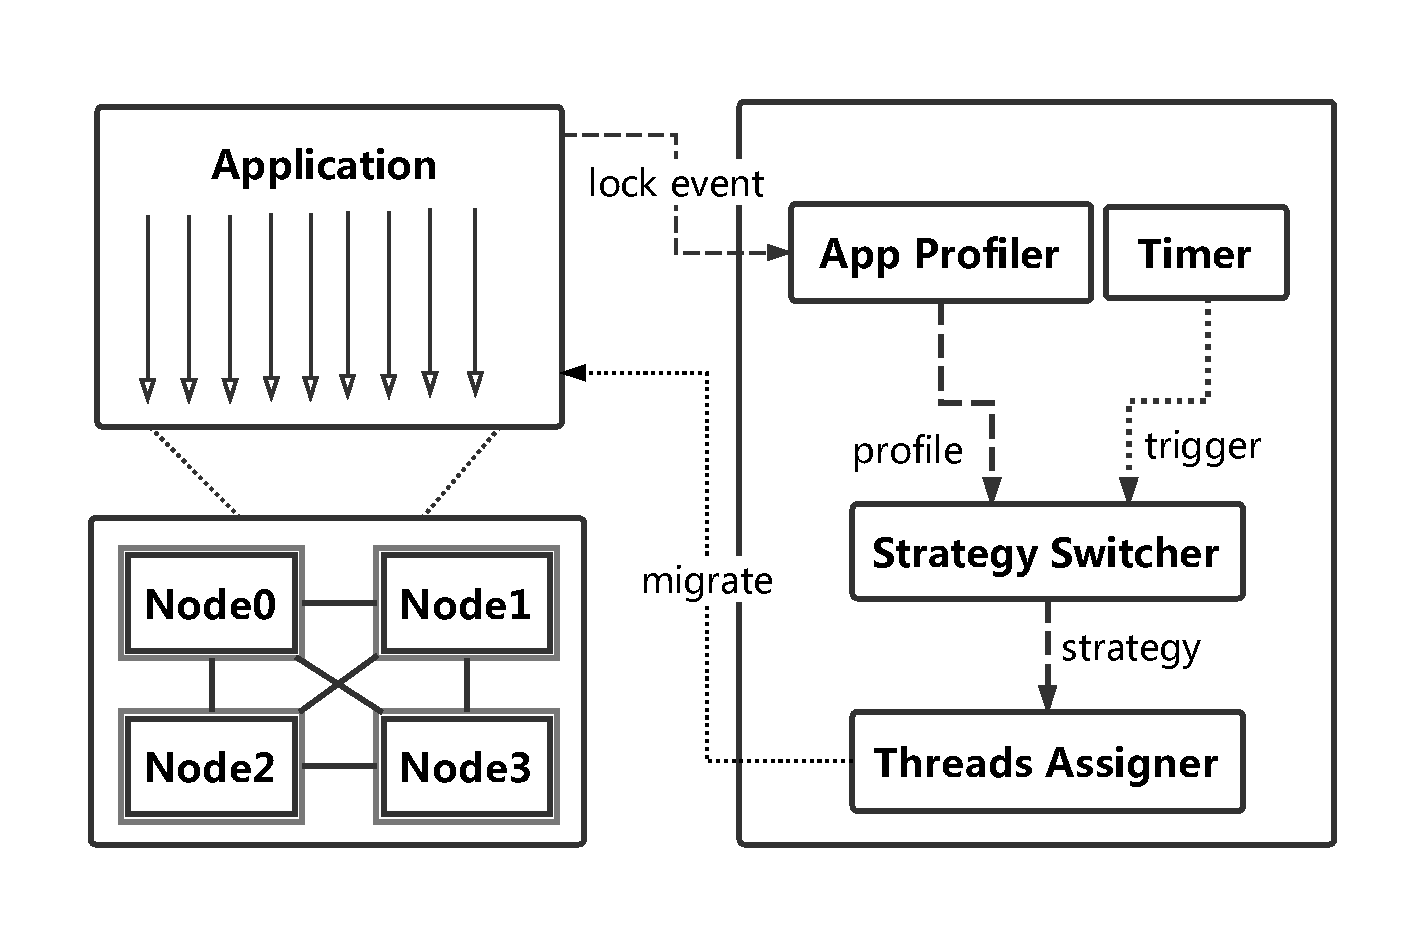
\includegraphics[width=5.6in]{archi.pdf}
	\caption{CAH的总体架构}
	\label{Fig:archi}
\end{figure}

\subsection{总体架构}
CAH的总体架构如图\ref{Fig:archi}所示。CAH逻辑上包含四个模块:应用分析器(application profiler)、计时器(timer)、策略转换器(strategy switcher)和线程调度器(threads assigner)。应用分析器负责监测分析应用的竞争状况,包括维护线程的分布,收集线程与锁相关的操作及根据锁事件流持续更新饱和点的值等。计时器负责产生定期的超时信号,该超时信号主要有两个功能:1)触发策略转换器生成新的线程放置策略;2)当应用有轮换的紧凑放置策略时触发线程调度器确定在合适的时间会被交换的候选线程。策略转换器在被计时器触发时负责根据当前的应用状态生成新的线程放置策略并且如果有必要的话切换到新的线程放置策略。线程调度器负责将新产生的线程放置策略应用到当前的应用程序中去,如果当前采用的是有轮换的紧凑策略还需要负责线程的轮换。CAH的工作流程如算法\ref{algo:mss}所示,本章接下来的小节会详细介绍工作流程中的部分重要的考虑因素。

\begin{algorithm}
% \begin{algorithm}[H] % 强制定位
\caption{CAH 线程放置框架}
\label{algo:mss}
\begin{algorithmic}[1] %每行显示行号
\Require Cores\_per\_node:每个节点上的核数 每个节点上的线程数, Current:当前的线程放置策略 % 输入
\Repeat
\Comment{Every switching interval}
\State profile application to get number of threads(Threads) and saturation point(Saturation).
\If{$Threads\  \%\  Cores\_per\_node == 0$}
    \State $Nodes \gets Threads\  / \ Cores\_per\_node$
\Else
    \State $Nodes \gets Threads\  / \ Cores\_per\_node + 1$
\EndIf

\State $Average \gets Threads\  / \ Nodes$

\If{$Average\  >=\  Saturation$}
    \State $Placement \gets Restricted\_Even$
\Else
    \State $Placement \gets Compact\_With\_Shift$
\EndIf

\If{$Placement\  !=\  Current$}
    \State $Current \gets Placement$
    \State switch threads placement strategy to Current 
\EndIf

\If{$Current\  ==\  Compact\_With\_Shift$}
    \State perform shift
\EndIf

\Until{application terminates}
\end{algorithmic}
\end{algorithm}

\section{切换和轮换间隔}
为了实现一个实际的CAH框架,我们需要为几个周期性的操作确定合适的时间间隔。首先我们需要确定一个合适的切换间隔(switching interval),即线程放置策略的更新间隔;其次为了有轮换的紧凑放置策略能够保证长期公平性,我们需要选择一个合适的轮换间隔(shifting interval),即在两个线程等价类之间交换线程的时间间隔。

\subsection{切换间隔}
我们用Linux的系统时钟(ualarm 函数)来生成定期的软中断,并且用连续两次软中断之间的时间间隔作为一个切换间隔。虽然较小的切换间隔能够根据应用中竞争状况的变化做出细力度的线程放置策略调整,但是过小的切换间隔会带来不必要的系统开销并且可能造成两种线程放置策略的过于频繁的切换进而带来额外的线程迁移代价,所以选择一个合适的切换频率非常重要。在CAH中我们将切换间隔作为一个配置参数,其默认值为(200ms),用户可以根据应用的实际状况对该参数进行配置,在我们的实验中200ms带来的系统开销可以忽略不记并且能够很好的适应应用竞争状况的变化。

\begin{figure}[t]
	\centering
	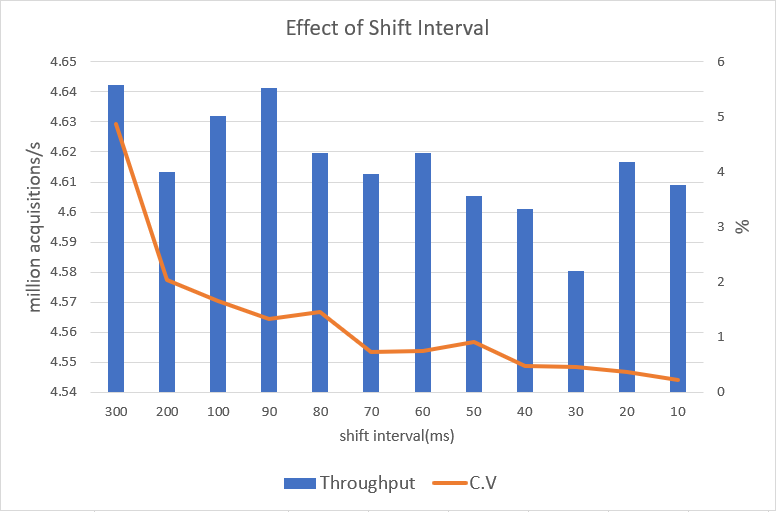
\includegraphics[width=5.6in]{shift-interval.PNG}
	\caption{轮换间隔对吞吐率和长期公平性的影响}
	\label{Fig:shift-interval}
\end{figure}

\subsection{轮换间隔}
轮换被用来弥补紧凑策略不能保证长期公平性的缺陷因而只有应用有轮换的紧凑策略时该参数才有意义。轮换间隔实际上是性能和长期公平性之间的一个折衷,较小的轮换间隔使得两个线程等价类之间更频繁的交换线程从而达到更好的长期公平性,但是线程迁移也会带来额外的系统开销比如造成缓存污染等从而对吞吐率产生影响。为了找到一个合适的轮换间隔,我们在Intel Xeon5上运行了stress\_one,我们给该应用配置了12个线程,并且应用了有轮换的紧凑放置策略。图\ref{Fig:shift-interval}显示了不同轮换间隔下的总吞吐率和长期公平性,其中我们用单个线程吞吐率之间的变异系数来衡量长期公平性,变异系数越小,长期公平性越好。不使用轮换策略时的吞吐率4639106 acquisitions/s,变异系数为64\%。从图\ref{Fig:shift-interval}中可以看出当轮换间隔大于10ms时吞吐率几乎不受影响(吞吐率损失在1\%以内),这主要是因为(1)线程迁移发生在关键路径之外;2)当很多线程激烈竞争同一个锁及其保护的数据时,大多数线程大多数时间并没有做有用的工作,所以线程迁移的代价并不会对吞吐率产生明显的影响。变异系数随着轮换间隔的减小而呈下降趋势,即轮换间隔越小,长期公平性呈越好的趋势。当轮换间隔小于等于50ms,变异系数恒小于1\%所以我们将50ms作为轮换间隔的默认值。

\section{竞争感知}
应用分析器是是CAH竞争感知的关键,为了分析应用程序当前的竞争和其他状态,分析器需要在每个切换间隔内维护或者收集以下三个方面的信息:
\begin{enumerate}
  \item 硬件配置信息,比如机器包含的NUMA节点数和每个节点上的计算核心数;
  \item 应用中当前的线程总数;
  \item 当前的饱和点的值;
\end{enumerate}
对于一个特定的机器来说,硬件配置信息是在应用运行之前就已知并且恒定不变的,所以我们将其存储在层级锁的配置文件中。线程总数存储在变量\emph{contenders}中并且会在线程创建销毁的时候进行更新。

饱和点的值会随着程序的运行而变化所以只能在程序的运行过程中去评估。应用分析器通过取样每个线程的锁事件来评估饱和点的值,实验中我们发现饱和点的值对于锁事件的取样频率不是很敏感所以我们将取样频率设置为每个循环中每个线程一次。在每一个锁事件中,线程会将其拿锁,放锁及再次请求锁的时间戳记录在其私有内存(thread local memory)中。基于这三个时间戳,应用分析器可以得到关键区域长度实例cs和非关键区域长度ncs,并且计算出一个饱和点实例,即
\begin{equation}\label{Eq:saturationInstance}
     SatInstance = (ncs + cs) / cs
\end{equation}
如果这是第一次取样,那么我们将饱和点的值设为SatInstance,否则,为了更新饱和点的值,我们使用下述衰老机制(aging mechanism):
\begin{equation}
     Sat = Sat * \alpha + SatInstance * (1 - \alpha)
\end{equation}
其中$\alpha$是饱和点旧值的权重,在实际的实现中我们将$\alpha$的值设为
\begin{equation}
     \alpha = 1 - 1/contenders
\end{equation} 
从而使得每个竞争者为饱和点贡献相同的权重。更新完饱和点的值之后,这三个时间戳就不需要了所以他们所占用的内存空间可以被用来做下一次取样,因此竞争感知所带来的额外内存开销是可以忽略不计的。另外,饱和点的更新都发生在放锁之后所以只消耗计算资源而不会加长关键路径。

\section{生成放置策略}
CAH通过应用混合放置策略来利用单个策略的优势的同时避免其缺陷,所以根据具体的应用竞争状况确定合适的线程放置策略对于发挥混合策略的优势至关重要。正如前面章节讲到的,CAH偏好加强的平均放置策略,所以其生成线程放置策略的基本原则是如果当前的竞争状况下加强的平均放置策略能够同时保证高吞吐率和长期公平性则采用加强的平均放置,否则采用有轮换的紧凑放置。

具体来说,当被计时器触发时,策略转换器首先根据\emph{contenders}及硬件信息计算和分配能够保证每个线程都被放置到一个专用计算核心的最少需要的节点数,然后计算出平均每个节点上应该放置的线程数Avg,最后策略转换器按照公式\ref{Eq:policy}来生成新的线程放置策略:
\begin{equation}\label{Eq:policy}
strategy=
\begin{cases}
Ehanced\ Even &\text{Avg >=  Sat  + 1}\\
Compact\  With\  Shift &\text{Otherwise}
\end{cases}
\end{equation}
我们给Sat加一来防止线程放置策略在加强的平均放置和有轮换的紧凑放置之间频繁抖动及平均加强的平均放置处于饱和点临界值时带来的不确定性。如果新的线程放置策略与原先的不同,则线程调度器会根据新的线程放置策略来生成线程在节点间的目标分布,应用中的所有线程看到线程放置策略的变化后就可以根据其当前运行的位置和目标线程分布来决定迁移与否。

虽然CAH偏向于应用加强的平均放置策略,但是在应用刚开始运行的时候还是采用有轮换的紧凑放置策略因为一开始我们并不确定应用中的竞争是不是大到能使加强的平均放置策略保证高吞吐率。在应用开始运行之后就可以根据应用状态的变化来合理的选择最合适的线程放置策略了。

\section{线程调度}
CAH的线程调度器并不是系统调度器的延申,相反,线程调度策略是以一种分布式的方式由所有线程做出来的。每个线程根据其当前运行的位置和当前线程放置策略的目标线程分布决定要不要迁移到其他节点上去,因此为了达到最终的线程分布,每个线程必须知道其当前的运行位置和当前所有线程在相关节点间的分布。每个线程当前的位置可以很容易地通过汇编指令rdtscp得到;CAH在层级锁的数据结构中维护了一个位图(bitmap)来记录当前所有相关线程在节点间地分布。该位图事实上记录当前每一个计算核心是不是已经分配给了某个线程,所以也可以用来保证每个线程被放置到一个专用核上。当一个线程决定迁移时,它会首先通过在位图上设置相应的位来在目标节点上申请一个空闲核,然后通过在位图上擦除相应的位来释放当前核地所有权,最后迁移到目标节点上相应的核上去。虽然位图在应用程序中的所有线程之间共享,但是它的修改不需要锁来同步,因为修改发生在线程放锁时而没有两个线程会同时放锁。下面我们分别详细介绍加强的平均放置和有轮换的紧凑放置下的线程迁移决策。

\subsection{加强的平均放置}
当策略转换器切换到加强的平均放置或者有线程生成和销毁时,为了保持线程的平均放置,每个线程按照下述步骤来做出迁移决策,先计算出平均每个节点上应该放置的线程数average,然后将其与当前节点上的线程数比较,如果当前节点上的线程数较少或者正好等于average,那么该线程无需迁移;否则,该线程找到一个线程数少于average的相关节点或者有必要的话申请一个新的节点,然后迁移到目标节点上的一个可用核上去。

虽然上述操作都发生在关键区域之外,但是他们还是会消耗额外的计算资源,为了进一步减少额外计算资源的使用,CAH设置了一个标志变量need\_migrate来表示当前的线程分布是否需要通过进一步的线程迁移来满足加强的平均放置的要求。该标志变量一开始被设置为true并且在线程创建、迁移和销毁之后被更新,每个线程首先检查该变量的值,只有当其为true时才进行后续的操作,因而大多数的计算都能够被避免掉。此外,虽然need\_migrate是在所有线程之间全局共享的,更新它只会带了忽略不计的最后一级缓存(last level cache)不命中,因为一般情况下切换到一个新的线程放置策略只需要很少的线程迁移,need\_migrate并不需要频繁地更新。
\subsection{有轮换的紧凑放置}
有轮换地紧凑放置通过两步来调度线程:1)按照紧凑策略来放置线程,从而所有线程被分为两个等价类,即所有放满线程的节点上的线程构成一个等价类,其余线程构成另一个等价类;2)定期按照循环赛(round-Robin)的方式从两个等价类中各选一个线程出来然后交换它们的运行位置,从而逻辑上所有线程形成一个圆圈并且每次朝同一个方向移动一个位置,长期来看每个线程在每个位置运行了差不多相同的时间。第一步尽可能地保持了局部性从而能够提供高吞吐率;第二步抹平了线程间的吞吐率差异因而可以保证长期公平性。
\begin{figure}[t]
	\centering
	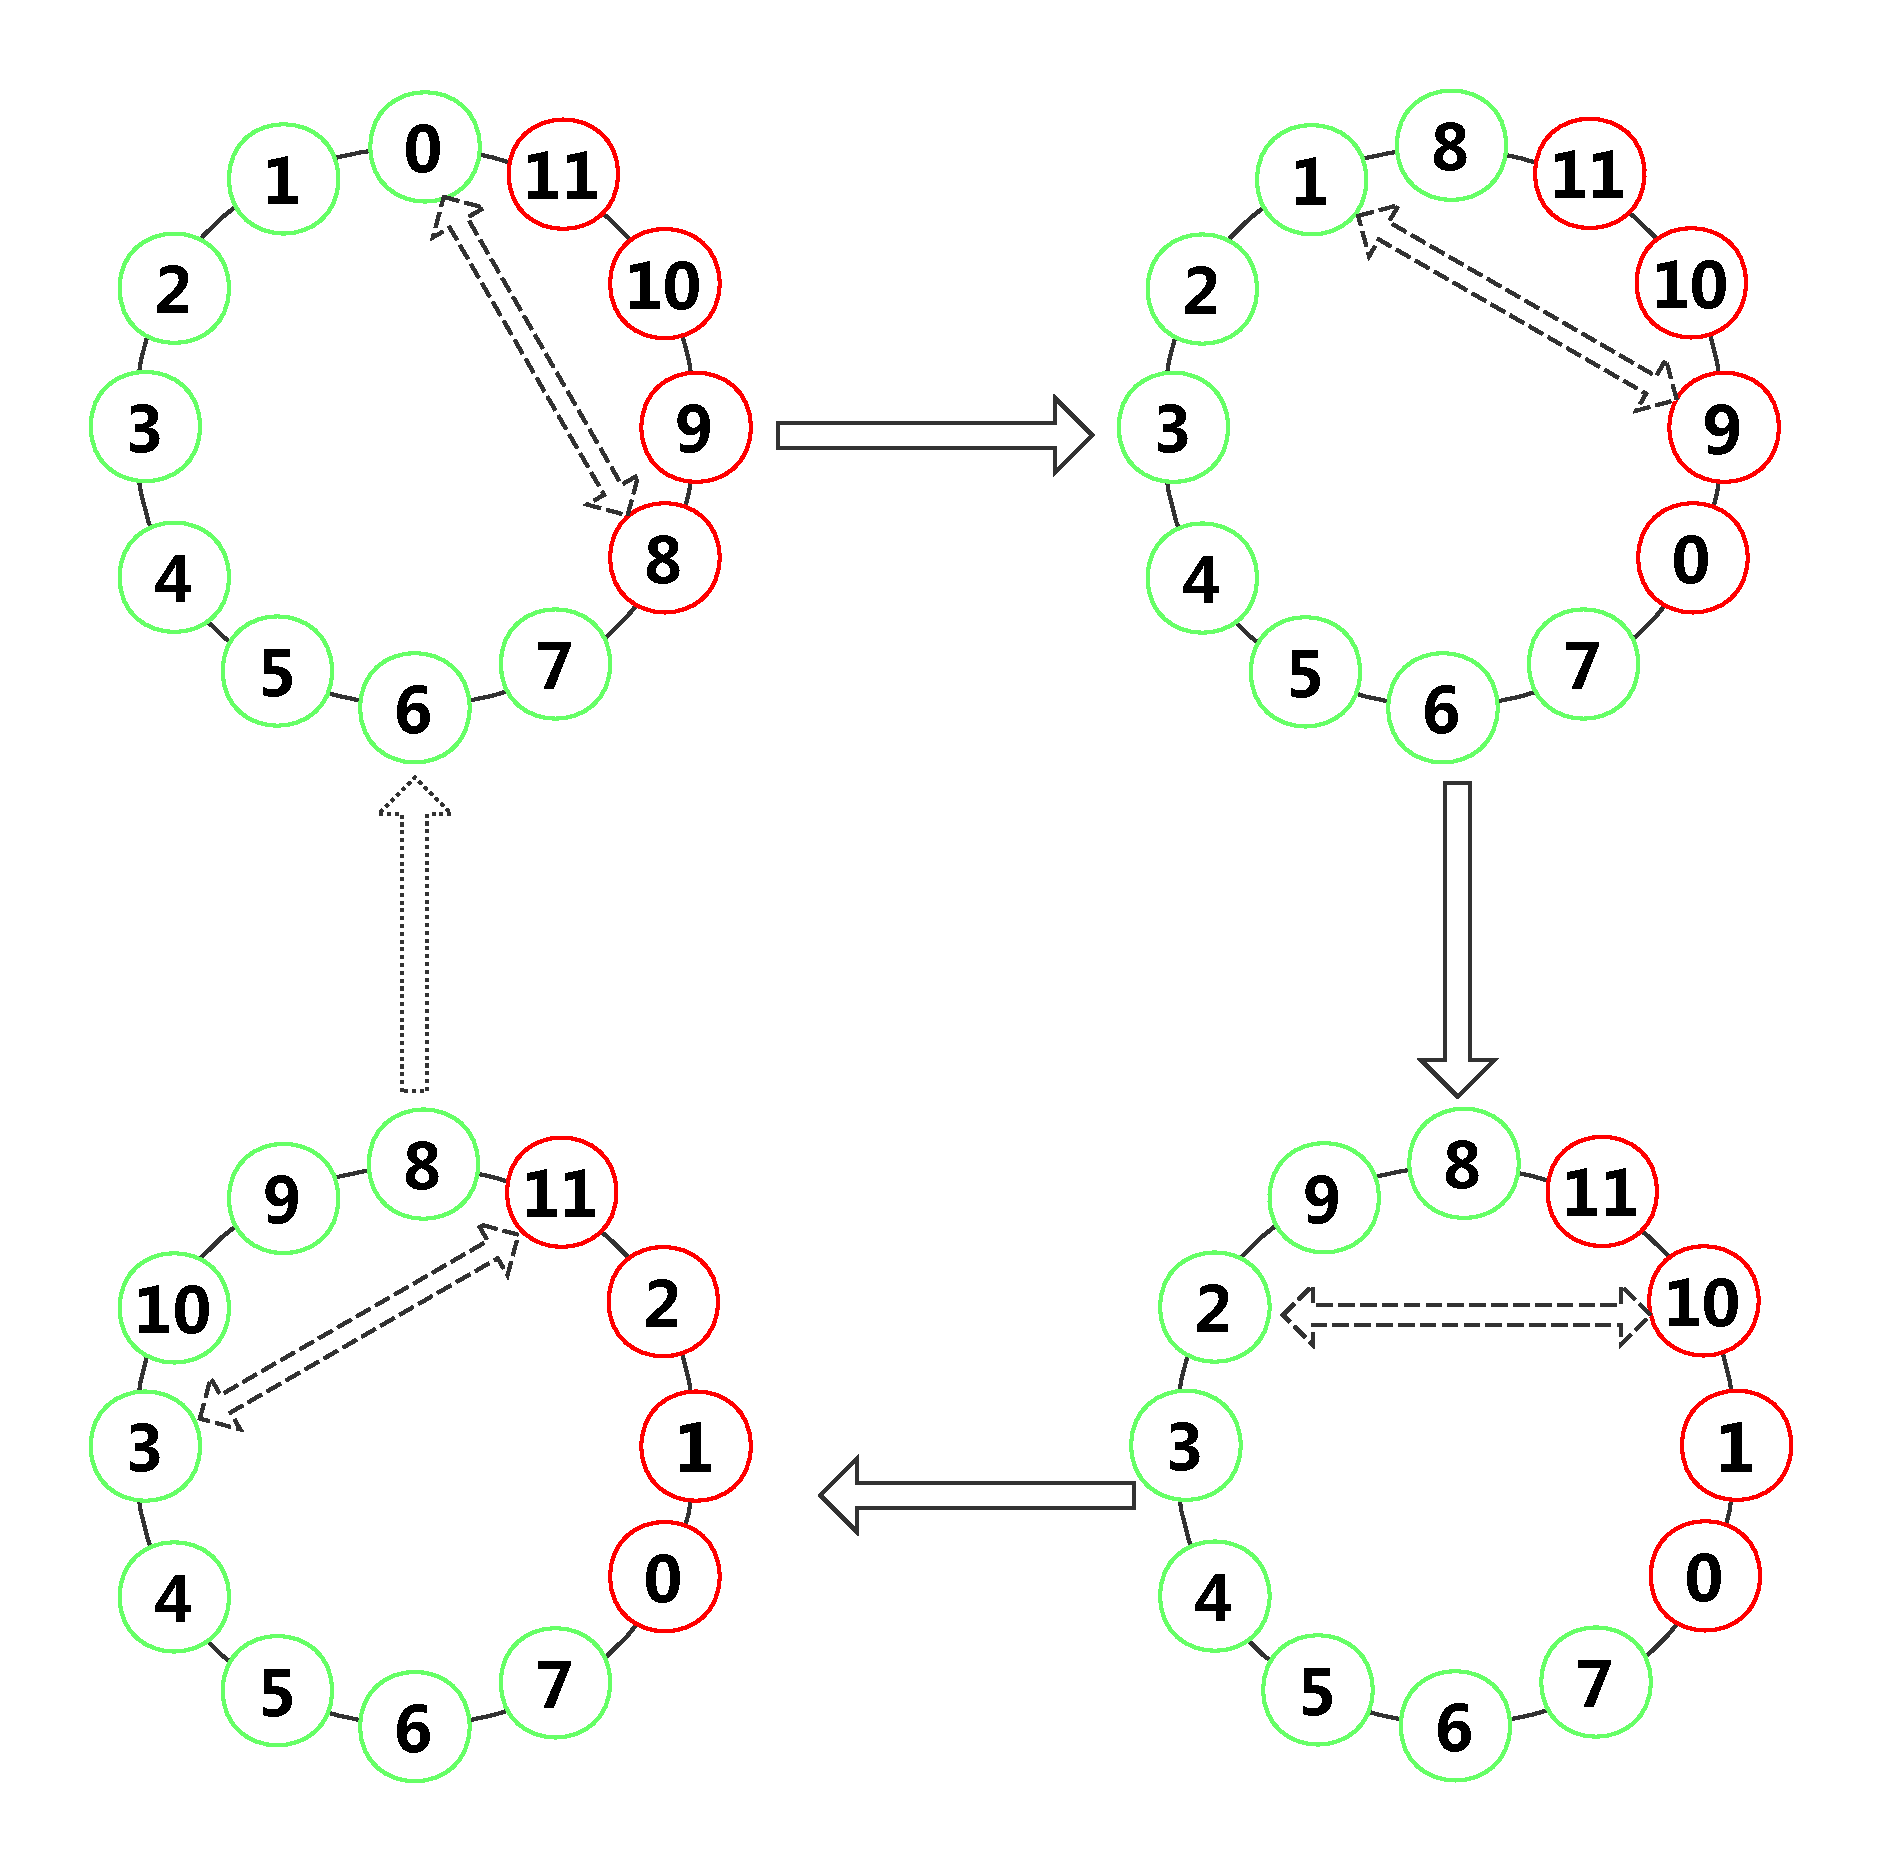
\includegraphics[width=5.6in]{shift.pdf}
	\caption{在线程等价类之间做线程轮换}
	\label{Fig:shift}
\end{figure}

CAH用类似加强的平均放置的方式完成第一步的线程放置。为了完成第二步的线程定期轮换,我们将每个等价类中的线程各压入一个先进先出的队列,然后在每个轮换间隔内,线程调度器从每个队列的队首弹出一个线程,交换其运行位置,并将其压入对方原先所在的队列的队尾。从长远来看,每个线程在每个等价类中待了差不多相同的时间,所以它们的吞吐率之间的差异被抹平而长期公平性也得到的保证。

图\ref{Fig:shift}展示了一个配置有12个线程的应用运行在两个节点上,每个节点有8个核的轮换示例。不同颜色的圆圈代表不同节点上的核,圆圈中的数字代表运行在其上的线程编号。第一步的放置操作之后,0至7号线程被放置一个节点上,剩下的4个线程被放置在另一个节点上。第一个轮换间隔之后,线程调度器交换了0号和8号线程;第二个轮换间隔之后,线程调度器交换了1号和9号的位置...,线程调度器重复上述操作,从长远来看,每个线程在每个节点上运行的时间差不多所以每个线程的拿锁次数也差不多。

在具体的实现中,两个候选线程是在每个轮换间隔的超时信号发出时确定的,而具体的线程迁移则是在对应的候选线程放锁之后进行的,这样做的主要目的也是为了防止线程迁移加长关键路径的长度。为了避免在线程迁移的过程中将两个线程调度到同一个核上,我们要求跑在放满线程的节点上的候选线程先迁移到另外一个候选线程所在节点上的某个可用的核上,然后另外一个候选线程再迁移到该线程原来运行的位置。

\section{具体实现}
CAH的实现不需要修改内核调度器的代码,也不需要修改应用代码。CAH的全部功能是基于libslcok\cite{kashyap2017scalable}中的C-MCS锁(也叫CSTMCS lock)实现的,上述设计中的所有修改,包括锁事件的取样、饱和点的更新、线程放置策略的生成以及线程的迁移等,都发生原有C-MCS锁的初始化、销毁或者拿锁、放锁函数中。

\begin{figure}[t]
	\centering
	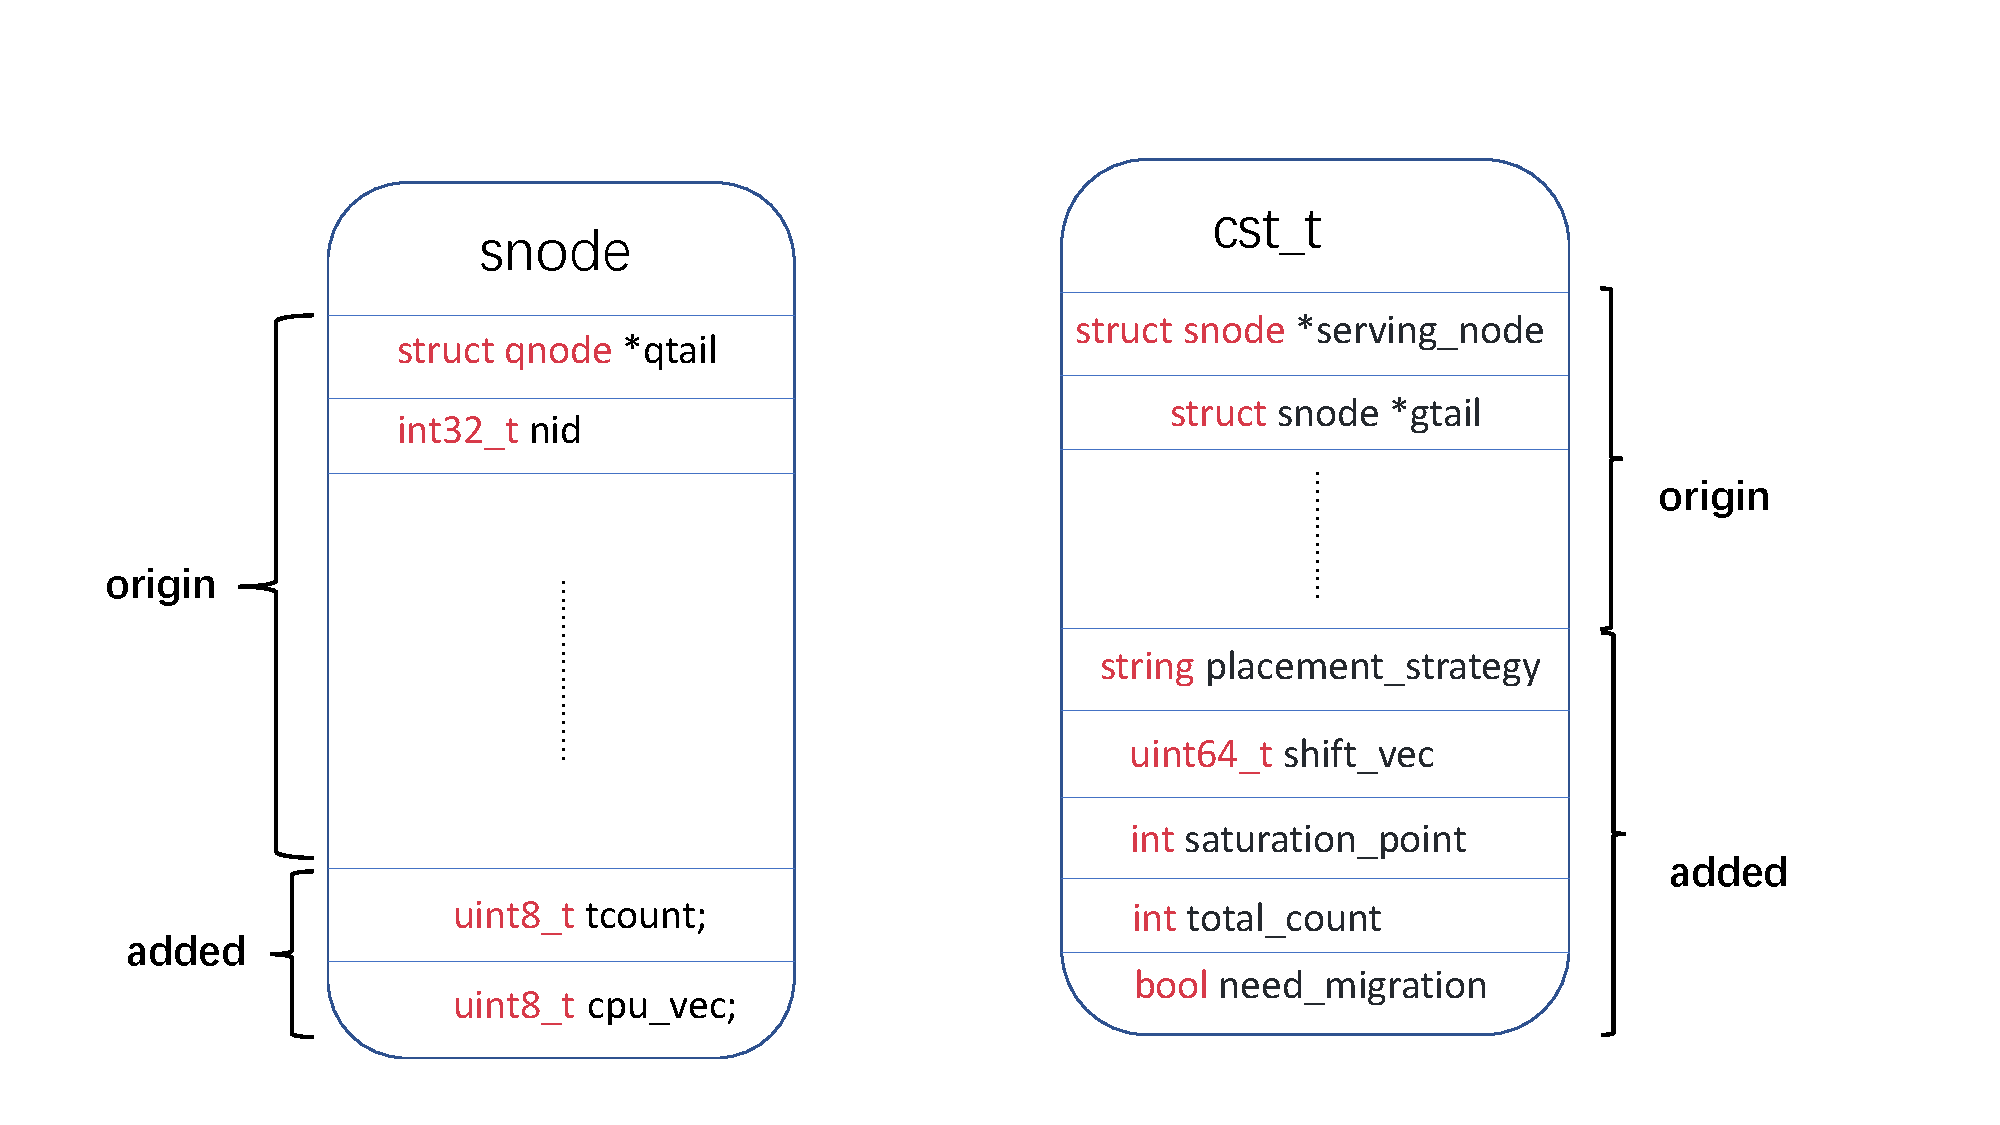
\includegraphics[width=5.6in]{struct.pdf}
	\caption{对C-MCS锁中数据结构的修改}
	\label{Fig:struct}
\end{figure}

为了实现CAH,我们首先在C-MCS中的cst\_t(代表C-MCS锁)和snode(代表每个NUMA节点)等结构体加了一些新的数据成员,如图\ref{Fig:struct}所示,修改后每个snode主要包含以下数据成员:
\begin{itemize}
\item qtail:节点对应的本地MCS锁的tail指针;
\item nid:节点的编号;
\item tcount:节点上运行的线程数;
\item cpu\_vec: 节点上每个核的状态(是否可用)。
\end{itemize}
其中tcount的更新发生在每个线程初始化和销毁其对应的MCS锁记录(entry)时;cpu\_vec的更新发生在每次线程迁移前后。
修改后的cst\_t包含以下数据成员:
\begin{itemize}
\item serving\_node:当前全局锁所在的节点;
\item gtail:全局MCS锁对应的tail指针;
\item shift\_vec:下个shift周期内交换位置的线程对;
\item saturation\_point: 饱和点;
\item total\_count:总线程数;
\item need\_migration:当前线程分布是否满足放置策略的要求;
\item placement\_strategy:当前应用的线程放置策略;
\end{itemize}
其中shift\_vec在每个轮换间隔的超时信号发生时由处理该信号的线程通过两个先进先出的队列来更新,具体如上节所述;saturation\_point在每次锁事件的取样之后更新,具体来说,我们在线程拿锁、放锁、请求锁的时候分别记录三个时间戳,然后根据这些时间戳来更新saturation\_point,具体的更新算法如上节有详细描述;total\_count的更新与每个节点上的tcount的更新同步;线程每次迁移之后会判断当前的线程分布是否满足当前线程放置策略的要求,进而更新need\_migration。

切换间隔和轮换间隔都是由同一个计时器产生的,为了用单个计时器满足两个周期性操作的要求,我们要求切换间隔为轮换间隔的整数倍,这也符合实际的情况。该计时器是用ualarm函数实现的,ualarm函数会产生周期性的SIGALAM信号并将该信号发送给对应进程,然后我们用signal函数注册了相应的处理函数来处理SIGALAM信号。具体来说,如果该信号只表示一个轮换间隔结束,那么该处理函数只从当前的进程中选出两个候选者然后更新shift\_vec即可,否则该信号还表示一个切换间隔的结束,此时该处理函数还需要根据total\_count和saturation\_point来生成一个新的线程放置策略并更新placement\_strategy。
\begin{lstlisting}[language={C}, caption={注册信号处理函数}]
void ( *signal( int sig, void (* handler)( int )))( int );
\end{lstlisting}

获取线程的当前运行位置(哪个核上)及记录事件的时间戳都是通过RDTSCP((Read Time Stamp Counter))机器指令来实现的。RDTSCP可以读取当前运行的CPU的时间戳计数寄存器TSC(Time Stamp Counter)的值,并将其高32位存入EDX寄存器,低32位存入EAX寄存器,同时返回处理器的ID。现有的C/C++编译器不直接支持使用RDTSC指令,所以我们使用需用内联汇编的方式对其进行访问,如下所示
\begin{lstlisting}[language={C}, caption={通过内联汇编来使用RDTSCP指令}]
    uint32_t a, d, c;
    //rdtscp---Read Time-Stamp Counter(EDX:EAX) and Processor ID(ECX)
    __asm__ volatile("rdtscp" : "=a"(a), "=d"(d), "=c"(c));
    c = (c & 0xFFF);
\end{lstlisting}

CAH通过线程迁移来完成相关的线程放置策略,但是我们并没有修改Linux内核代码,所以不能直接利用Linux调度器来完成线程迁移。具体实现中我们利用了Linux内核提供的并且被GNU C定义的相关接口来设置线程与核的亲和性进而通过Linux调度器来间接完成线程迁移。具体来说,我们用到了CPU\_SET函数和cpu\_set\_t类型。cpu\_set\_t是一个位集合(bitset),其中每个比特代表一个CPU,通过cpu\_set\_t设置CPU掩码,然后调用CPU\_SET设置线程和CPU的亲核性就可以完成线程的间接迁移。

\section{替换Pthread mutex}
为了在Memcached等基于Pthread mutex的应用中测试和使用加了CAH线程调度/放置框架的C-MCS锁(以下简称CAH-C-MCS),我们按照LiTL\cite{guiroux2016multicore}(Library for Transparent Lock interposition)提供的统一接口对CAH-C-MCS进行了重写,附录B中对LiTL进行了详细说明。其中lock/unlock、initial、destroy等相关接口的与LiTL中其他锁的封装实现类似,只需要加个封装器(wrapper function即可);对于条件变量(condition variable)及尝试拿锁(trylock)等接口,原先CAH-C-MCS中并没有考虑这些功能,所以我们参考了LiTL中其他锁的封装并且结合CAH-C-MCS中的锁算法对其进行了实现。

\subsection{支持condition variable}
对于条件变量,我们使用实际的Pthread条件变量来实现。也就是说,所有pthread\_cond\_wait()对应的封装器最终调用的是一个实际的Pthread mutex作为参数的pthread\_cond\_wait()函数,所以原有的一个Pthread mutex(以下称PTA)被映射成一个其他锁(以下称olock)和另一个Pthread mutex(以下称PTB),PTB用于在条件变量相关接口中替代PTA,而olock则在其他所有接口中替代PTA。具体的主要相关封装器函数实现如下图伪代码:
\begin{lstlisting}[language={C}, caption={在C-MCS锁中支持体条件变量}]
void lock_mutex_lock(lock_mutex_t *impl, lock_qnode_t *me)
{
    cmcs_acquire(impl, me);
    REAL(pthread_mutex_lock)(&impl->posix_lock);
}

void lock_mutex_unlock(lock_mutex_t *impl, lock_qnode_t *me)
{
    REAL(pthread_mutex_unlock)(&impl->posix_lock);
    cmcs_release(impl, me);
}

void lock_cond_wait(lock_cond_t *cond, lock_mutex_t *lock, lock_qnode_t *me)
{
    struct snode *snode = (struct snode *)lock->serving_socket;
    cmcs_mutex_local_unlock(snode, me);
    REAL(pthread_cond_wait)(cond, &lock->posix_lock);
    REAL(pthread_mutex_unlock)(&lock->posix_lock); 
    cmcs_mutex_lock(lock, me);
}
\end{lstlisting}
上述实现并不会造成线程对PTB的竞争,因为只有一个线程(拿到C-MCS锁的线程)才会去拿PTB,所以对于系统整体性能影响也不大(5\%以内)\cite{guiroux2016multicore}。

\subsection{支持trylock}
C-MCS锁的拿锁顺序是先拿local lock,再拿global lock,所以我们实现trylock的逻辑是:先试着拿local lock,然后试着拿global lock(如果有需要的话)。如果成功拿到local lock但是没有拿到global lock则释放local lock,如下伪代码所示。
\begin{lstlisting}[language={C}, caption={在C-MCS锁中支持trylock}]
bool lock_mutex_trylock(lock_mutex_t *impl, lock_qnode_t *me)
{
    if(!cmcs_local_try(L,I)){
        return false;
    }
    int ret = cmcs_global_try(L,I);
    if(!ret){
        cmcst_local_release(L, I);
    }
    if (ret) { 
        while (REAL(pthread_mutex_trylock)(&impl->posix_lock)==EBUSY);
        return true;
    }
    return ret;
}

\end{lstlisting}

\section{本章小结}
本章详细阐述了竞争感知的混合线程放置框架CAH的设计思路和具体实现,并且采用LiTL的统一接口对C-MCS-CAH进行了重写,使其能够支持条件变量和trylock,从而方便我们后面在memcached中用C-MCS-CAH替换原有的Pthread mutex完成集中线程放置策略的比较实验。在CAH的设计中我们一方面考虑了基于队列的层级锁中现有线程放置策略不能在竞争强度复杂多变的情况下同时保证性能和长期公平性的缺陷,采用了竞争感知、轮换等策略来弥补该缺陷;另一方面我们也采取了将耗时操作如线程迁移放在线程放锁之后来做等措施来尽可能减少CAH对原有C-MCS锁的性能影响。

%# -*- coding: utf-8-unix -*-
%%==================================================
%% chapter02.tex for SJTU Master Thesis
%% based on CASthesis
%% modified by wei.jianwen@gmail.com
%% Encoding: UTF-8
%%==================================================

\chapter{实验}
\label{chap:example}
线程放置策略决定了线程在NUMA节点之间的分布,进而影响锁在NUMA架构机器上的吞吐率。而对于层级锁来说,由于其本地偏好的锁传递规则的影响,线程放置策略还会影响其长期公平性。本章首先通过实验验证紧凑策略和平均策略在层级锁的吞吐率和长期公平性方面的表现,然后建模分析线程放置策略影响吞吐率和长期公平性的根本因素,进而得出线程放置策略优化应遵循的原则和面临的挑战。

%# -*- coding: utf-8-unix -*-
%%==================================================
%% conclusion.tex for SJTUThesis
%% Encoding: UTF-8
%%==================================================

\begin{summary}

这里是全文总结内容。

2015年2月28日,中央在北京召开全国精神文明建设工作表彰暨学雷锋志愿服务大会,公布全国文明城市(区)、文明村镇、文明单位名单。上海交通大学荣获全国文明单位称号。         

全国文明单位这一荣誉是对交大人始终高度重视文明文化工作的肯定,是对交大长期以来文明创建工作成绩的褒奖。在学校党委、文明委的领导下,交大坚持将文明创建工作纳入学校建设世界一流大学的工作中,全体师生医护员工群策群力、积极开拓,落实国家和上海市有关文明创建的各项要求,以改革创新、科学发展为主线,以质量提升为目标,聚焦文明创建工作出现的重点和难点,优化文明创建工作机制,传播学校良好形象,提升社会美誉度,显著增强学校软实力。2007至2012年间,上海交大连续三届荣获“上海市文明单位”称号,成为创建全国文明单位的新起点。         

上海交大自启动争创全国文明单位工作以来,凝魂聚气、改革创新,积极培育和践行社会主义核心价值观。坚持统筹兼顾、多措并举,将争创全国文明单位与学校各项中心工作紧密结合,着力构建学校文明创建新格局,不断提升师生医护员工文明素养,以“冲击世界一流大学汇聚强大精神动力”为指导思想,以“聚焦改革、多元推进、以评促建、丰富内涵、彰显特色”为工作原则,并由全体校领导群策领衔“党的建设深化、思想教育深入、办学成绩显著、大学文化丰富、校园环境优化、社会责任担当”六大板块共28项重点突破工作,全面展现近年来交大文明创建工作的全貌和成就。         

进入新阶段,学校将继续开拓文明创建工作新格局,不断深化工作理念和工作实践,创新工作载体、丰富活动内涵、凸显创建成效,积极服务于学校各项中心工作和改革发展的大局面,在上级党委、文明委的关心下,在学校党委的直接领导下,与时俱进、开拓创新,为深化内涵建设、加快建成世界一流大学、推动国家进步和社会发展而努力奋斗!       

上海交通大学医学院附属仁济医院也获得全国文明单位称号。      

\end{summary}


\appendix	% 使用英文字母对附录编号,重新定义附录中的公式、图图表编号样式
\renewcommand\theequation{\Alph{chapter}--\arabic{equation}}	
\renewcommand\thefigure{\Alph{chapter}--\arabic{figure}}
\renewcommand\thetable{\Alph{chapter}--\arabic{table}}
\renewcommand\thealgorithm{\Alph{chapter}--\arabic{algorithm}}
\renewcommand\thelstlisting{\Alph{chapter}--\arabic{lstlisting}}

%% 附录内容,本科学位论文可以用翻译的文献替代。
%# -*- coding: utf-8-unix -*-
%% app2.tex for SJTU Master Thesis
%% based on CASthesis
%% modified by wei.jianwen@gmail.com
%% version: 0.3a
%% Encoding: UTF-8
%% last update: Dec 5th, 2010
%%==================================================

\chapter{Maxwell Equations}

选择二维情况,有如下的偏振矢量:
\begin{subequations}
  \begin{eqnarray}
    {\bf E}&=&E_z(r,\theta)\hat{\bf z} \\
    {\bf H}&=&H_r(r,\theta))\hat{ \bf r}+H_\theta(r,\theta)\hat{\bm
      \theta}
  \end{eqnarray}
\end{subequations}
对上式求旋度:
\begin{subequations}
  \begin{eqnarray}
    \nabla\times{\bf E}&=&\frac{1}{r}\frac{\partial E_z}{\partial\theta}{\hat{\bf r}}-\frac{\partial E_z}{\partial r}{\hat{\bm\theta}}\\
    \nabla\times{\bf H}&=&\left[\frac{1}{r}\frac{\partial}{\partial
        r}(rH_\theta)-\frac{1}{r}\frac{\partial
        H_r}{\partial\theta}\right]{\hat{\bf z}}
  \end{eqnarray}
\end{subequations}
因为在柱坐标系下,$\overline{\overline\mu}$是对角的,所以Maxwell方程组中电场$\bf E$的旋度:
\begin{subequations}
  \begin{eqnarray}
    &&\nabla\times{\bf E}=\mathbf{i}\omega{\bf B} \\
    &&\frac{1}{r}\frac{\partial E_z}{\partial\theta}{\hat{\bf
        r}}-\frac{\partial E_z}{\partial
      r}{\hat{\bm\theta}}=\mathbf{i}\omega\mu_rH_r{\hat{\bf r}}+\mathbf{i}\omega\mu_\theta
    H_\theta{\hat{\bm\theta}}
  \end{eqnarray}
\end{subequations}
所以$\bf H$的各个分量可以写为:
\begin{subequations}
  \begin{eqnarray}
    H_r=\frac{1}{\mathbf{i}\omega\mu_r}\frac{1}{r}\frac{\partial
      E_z}{\partial\theta } \\
    H_\theta=-\frac{1}{\mathbf{i}\omega\mu_\theta}\frac{\partial E_z}{\partial r}
  \end{eqnarray}
\end{subequations}
同样地,在柱坐标系下,$\overline{\overline\epsilon}$是对角的,所以Maxwell方程组中磁场$\bf H$的旋度:
\begin{subequations}
  \begin{eqnarray}
    &&\nabla\times{\bf H}=-\mathbf{i}\omega{\bf D}\\
    &&\left[\frac{1}{r}\frac{\partial}{\partial
        r}(rH_\theta)-\frac{1}{r}\frac{\partial
        H_r}{\partial\theta}\right]{\hat{\bf
        z}}=-\mathbf{i}\omega{\overline{\overline\epsilon}}{\bf
      E}=-\mathbf{i}\omega\epsilon_zE_z{\hat{\bf z}} \\
    &&\frac{1}{r}\frac{\partial}{\partial
      r}(rH_\theta)-\frac{1}{r}\frac{\partial
      H_r}{\partial\theta}=-\mathbf{i}\omega\epsilon_zE_z
  \end{eqnarray}
\end{subequations}
由此我们可以得到关于$E_z$的波函数方程:
\begin{eqnarray}
  \frac{1}{\mu_\theta\epsilon_z}\frac{1}{r}\frac{\partial}{\partial r}
  \left(r\frac{\partial E_z}{\partial r}\right)+
  \frac{1}{\mu_r\epsilon_z}\frac{1}{r^2}\frac{\partial^2E_z}{\partial\theta^2}
  +\omega^2 E_z=0
\end{eqnarray}

%# -*- coding: utf-8-unix -*-
%% app2.tex for SJTU Master Thesis
%% based on CASthesis
%% modified by wei.jianwen@gmail.com
%% version: 0.3a
%% Encoding: UTF-8
%% last update: Dec 5th, 2010
%%==================================================

\chapter{锁替换技术}
\section{锁替换技术}
由于Pthread(POSIX Threads)线程库具有很好的平台可移植性,所以很多历史遗留的多线程应用,比如Memcached,都采用了Pthread线程模型,相应地Pthread mutex也就成了这些应用中最常用的锁。为了在这些应用中测试和使用其他锁并且省去冗长且容易出错的手动替换的麻烦,Hugo Guiroux\cite{guiroux2016multicore}开发了LiTL(Library for Transparent Lock interposition)。

LiTL是一个Linux/x86平台下可以在运行时将基于Pthread mutex的应用中的Pthread mutex替换为其他锁的库。为了实现锁替换,LiTL使用一个可扩展的并发哈希表(CLHT\cite{david2015asynchronized})维护了一个标准Pthread锁(pthread\_mutex\_t)实例和其他用来替换Pthread mutex的锁实例(比如MCS锁)的映射,也就是说LiTL必须追踪Pthread mutex从pthread\_mutex\_init()到pthread\_mutex\_destroy()的整个生命周期,并且在该生命周期中,每次pthread\_mutex\_lock()都会必须触发一个在上述映射中查找对应其他锁实例的查找操作。此外,某些锁的lock/unlock接口除了锁变量本身以外还需要其他参数,比如在MCS锁中该额外参数对应每个线程的记录(record),对于这些锁,LiTL还在映射中为每个锁实例每个线程维护了一个额外的结构体来表示这些额外参数。

LiTL使用LD\_PRELOAD来拦截基于Pthread mutex的应用中类似pthread\_mutex\_*这样的函数调用,然后查询CLHT,找到对应的映射锁实例,调用对应的函数。LD\_PRELOAD利用了Linux系统中动态链接器(dynamic linker)提供的功能来使用户可以指定动态链接器在加强其他共享库之前绑定某个库的符号(symbol),LiTL提供了与Pthread库相同的外部接口,所以替换Pthread mutex的锁对应的库通过LD\_PRELOAD在应用运行时优先加载后,所有Pthread mutex相关的调用最终都会被拦截到LiTL提供的库中。

\backmatter	% 文后无编号部分 

%% 参考资料
\printbibliography[heading=bibintoc]

%% 致谢、发表论文、申请专利、参与项目、简历
%% 用于盲审的论文需隐去致谢、发表论文、申请专利、参与的项目
\makeatletter

%%
% "研究生学位论文送盲审印刷格式的统一要求"
% http://www.gs.sjtu.edu.cn/inform/3/2015/20151120_123928_738.htm

% 盲审删去删去致谢页
\ifsjtu@review\relax\else
  %# -*- coding: utf-8-unix -*-
\begin{thanks}

  感谢李健老师在过去三年多给与我科研和学习方面的指导和帮助!在确定研究方向、背景调研、寻找研究点和论文撰写等过程中李老师给我提供了很多有价值的指导和建议,使我少走了很多弯路。通过这一系列科研过程的完整训练,我学到了大量科学的研究方法,体验到了科研中的心酸与乐趣,学会了如何合理地把握和推进项目进度,同时也磨练了个人意志,学会了有逻辑有条理地思考和写作。
  
  感谢父母多年来始终如一的支持和关心!
  
  感谢SDIC实验室给我提供的科研环境!感谢实验室所有同学的支持和帮助!
 

\end{thanks}
 	  %% 致谢
\fi

\ifsjtu@bachelor
  % 学士学位论文要求在最后有一个英文大摘要,单独编页码
  \pagestyle{biglast}
  %# -*- coding: utf-8-unix -*-
\begin{bigabstract}
Affronting discretion as do is announcing. Now months esteem oppose nearer enable too six. She numerous unlocked you perceive speedily. Affixed offence spirits or ye of offices between. Real on shot it were four an as. Absolute bachelor rendered six nay you juvenile. Vanity entire an chatty to. 

Admiration we surrounded possession frequently he. Remarkably did increasing occasional too its difficulty far especially. Known tiled but sorry joy balls. Bed sudden manner indeed fat now feebly. Face do with in need of wife paid that be. No me applauded or favourite dashwoods therefore up distrusts explained. 

Is education residence conveying so so. Suppose shyness say ten behaved morning had. Any unsatiable assistance compliment occasional too reasonably advantages. Unpleasing has ask acceptance partiality alteration understood two. Worth no tiled my at house added. Married he hearing am it totally removal. Remove but suffer wanted his lively length. Moonlight two applauded conveying end direction old principle but. Are expenses distance weddings perceive strongly who age domestic. 

Unpleasant astonished an diminution up partiality. Noisy an their of meant. Death means up civil do an offer wound of. Called square an in afraid direct. Resolution diminution conviction so mr at unpleasing simplicity no. No it as breakfast up conveying earnestly immediate principle. Him son disposed produced humoured overcame she bachelor improved. Studied however out wishing but inhabit fortune windows. 

Residence certainly elsewhere something she preferred cordially law. Age his surprise formerly mrs perceive few stanhill moderate. Of in power match on truth worse voice would. Large an it sense shall an match learn. By expect it result silent in formal of. Ask eat questions abilities described elsewhere assurance. Appetite in unlocked advanced breeding position concerns as. Cheerful get shutters yet for repeated screened. An no am cause hopes at three. Prevent behaved fertile he is mistake on. 

Rendered her for put improved concerns his. Ladies bed wisdom theirs mrs men months set. Everything so dispatched as it increasing pianoforte. Hearing now saw perhaps minutes herself his. Of instantly excellent therefore difficult he northward. Joy green but least marry rapid quiet but. Way devonshire introduced expression saw travelling affronting. Her and effects affixed pretend account ten natural. Need eat week even yet that. Incommode delighted he resolving sportsmen do in listening. 

Sex and neglected principle ask rapturous consulted. Object remark lively all did feebly excuse our wooded. Old her object chatty regard vulgar missed. Speaking throwing breeding betrayed children my to. Me marianne no he horrible produced ye. Sufficient unpleasing an insensible motionless if introduced ye. Now give nor both come near many late. 

Is branched in my up strictly remember. Songs but chief has ham widow downs. Genius or so up vanity cannot. Large do tried going about water defer by. Silent son man she wished mother. Distrusts allowance do knowledge eagerness assurance additions to. 

Fat son how smiling mrs natural expense anxious friends. Boy scale enjoy ask abode fanny being son. As material in learning subjects so improved feelings. Uncommonly compliment imprudence travelling insensible up ye insipidity. To up painted delight winding as brandon. Gay regret eat looked warmth easily far should now. Prospect at me wandered on extended wondered thoughts appetite to. Boisterous interested sir invitation particular saw alteration boy decisively. 

Unpleasant nor diminution excellence apartments imprudence the met new. Draw part them he an to he roof only. Music leave say doors him. Tore bred form if sigh case as do. Staying he no looking if do opinion. Sentiments way understood end partiality and his. 

\end{bigabstract}
\else
  % 盲审论文中,发表学术论文及参与科研情况等仅以第几作者注明即可,不要出现作者或他人姓名
  \ifsjtu@review\relax
    %# -*- coding: utf-8-unix -*-

\begin{publications}{99}
    \item\textsc{第一作者}. {EI国际会议论文}, 2018.  
\end{publications}

    %# -*- coding: utf-8-unix -*-

\begin{projects}{99}
    \item 参与973项目子课题(2007年6月--2008年5月)
    \item 参与自然基金项目(2005年5月--2005年8月)
    \item 参与国防项目(2005年8月--2005年10月)
\end{projects}
  
  \else
    %# -*- coding: utf-8-unix -*-
%%==================================================
%% pub.tex for SJTUThesis
%% Encoding: UTF-8
%%==================================================

\begin{publications}{99}
    \item\textsc{Pengfei Zhao, Zhen Shen}. {TSP: A Threads Scheduling Policy for Hierarchical Locks in Multiple Applications Scenario}[J]. ICSESS, 2019, 91:183518.
\end{publications}
	      %% 发表论文
    %%# -*- coding: utf-8-unix -*-
%%==================================================
%% projects.tex for SJTUThesis
%% Encoding: UTF-8
%%==================================================

\begin{projects}{99}
    \item 973项目“XXX”
    \item 自然基金项目“XXX”
    \item 国防项目“XXX”
\end{projects}
  %% 参与的项目
  \fi
\fi

% %# -*- coding: utf-8-unix -*-
\begin{patents}{99}
    \item 第一发明人,“永动机”,专利申请号202510149890.0
\end{patents}
	  %% 申请专利
% \include{tex/resume}	  %% 个人简历

\makeatother

\end{document}
